\documentclass[11pt]{book}
\usepackage[utf8]{inputenc}
\usepackage[english]{babel}
\usepackage{amsmath}
\usepackage{amssymb}
\usepackage{listings}
\usepackage{xcolor}
\usepackage{geometry}
\usepackage{fancyhdr}
\usepackage{graphicx}
\usepackage{tikz}
\usepackage{enumitem}

% Geometry settings
\geometry{margin=1in, headheight=14pt}

% Code listing style for Slate
\lstdefinestyle{slate}{
    basicstyle=\ttfamily\small,
    keywordstyle=\color{blue}\bfseries,
    keywordstyle=[2]\color{purple}\bfseries,
    keywordstyle=[3]\color{teal}\bfseries,
    keywordstyle=[4]\color{orange!80!black},
    keywordstyle=[5]\color{violet}\bfseries,
    commentstyle=\color{gray}\itshape,
    stringstyle=\color{red},
    numberstyle=\tiny\color{gray},
    identifierstyle=\color{black},
    breaklines=true,
    breakatwhitespace=true,
    tabsize=4,
    showspaces=false,
    showstringspaces=false,
    frame=single,
    rulecolor=\color{black!30},
    backgroundcolor=\color{gray!5},
    keywords={def, val, var, if, then, else, elif, end, and, or, not, match, case, default, while, do, for, loop, break, continue, return, import, package},
    keywords=[2]{true, false, null, undefined, NaN, Infinity},
    keywords=[3]{print, abs, sqrt, floor, ceil, sin, cos, tan, exp, ln, max, min, type, input, random},
    literate={//}{{{\color{orange!80!black}//}}}2
             {**}{{{\color{orange!80!black}**}}}2
             {==}{{{\color{orange!80!black}==}}}2
             {!=}{{{\color{orange!80!black}!=}}}2
             {<=}{{{\color{orange!80!black}<=}}}2
             {>=}{{{\color{orange!80!black}>=}}}2
             {+=}{{{\color{orange!80!black}+=}}}2
             {-=}{{{\color{orange!80!black}-=}}}2
             {*=}{{{\color{orange!80!black}*=}}}2
             {/=}{{{\color{orange!80!black}/=}}}2
             {&&}{{{\color{orange!80!black}\&\&}}}2
             {||}{{{\color{orange!80!black}||{}}}}2,
    otherkeywords={+, -, *, /, \%, <, >, =, !},
    morekeywords=[4]{+, -, *, /, \%, <, >, =, !},
    keywords=[5]{Array, String, Buffer, Object, Date, Duration, Period}
}

% Define Slate keywords
\lstset{
    morekeywords={def, val, var, if, then, else, elif, end, and, or, not, true, false, null, undefined, match, case, default},
    morecomment=[l]{\\}
}

\lstset{style=slate}

% Define a command for inline Slate code
\newcommand{\slate}[1]{\lstinline[basicstyle=\ttfamily,mathescape=true]{#1}}

% Plain style for syntax templates (no highlighting)
\lstdefinestyle{plain}{
    basicstyle=\ttfamily\small,
    frame=single,
    rulecolor=\color{black!30},
    backgroundcolor=\color{gray!5},
    breaklines=true,
    showspaces=false,
    showstringspaces=false,
    language={},
    keywordstyle={},
    commentstyle={},
    stringstyle={},
    identifierstyle={},
    keywords={},
    mathescape=true
}

% Page style
\pagestyle{fancy}
\fancyhf{}
\fancyhead[LE,RO]{\thepage}
\fancyhead[LO]{\nouppercase{\rightmark}}
\fancyhead[RE]{\nouppercase{\leftmark}}

\title{Structure and Interpretation of Computer Programs\\
\large Slate Edition}
\author{Adapted for the Slate Programming Language}
\date{\today}

\begin{document}

\maketitle

\newpage

\vspace*{\fill}

\noindent
\textbf{Copyright Notice}

\vspace{0.5cm}

\noindent
This work is based on \textit{Structure and Interpretation of Computer Programs} (Second Edition) by Harold Abelson, Gerald Jay Sussman, and Julie Sussman, published by MIT Press. The original work is licensed under a Creative Commons Attribution-ShareAlike 4.0 International License.

\vspace{0.3cm}

\noindent
Original work: \textit{Structure and Interpretation of Computer Programs} \\
Authors: Harold Abelson, Gerald Jay Sussman, and Julie Sussman \\
Publisher: MIT Press \\
License: Creative Commons Attribution-ShareAlike 4.0 International (CC BY-SA 4.0)

\vspace{0.3cm}

\noindent
This Slate Edition adaptation is also licensed under the Creative Commons Attribution-ShareAlike 4.0 International License. You are free to share and adapt this material under the terms of this license.

\vspace{0.3cm}

\noindent
License details: \texttt{https://creativecommons.org/licenses/by-sa/4.0/}

\vspace*{\fill}

\tableofcontents

\chapter{Building Abstractions with Procedures}

% Programming in Slate introduction section
\section*{Programming in Slate}
\addcontentsline{toc}{section}{Programming in Slate}

We need an appropriate language for describing processes, and we will use for this purpose the programming language Slate. Just as our everyday thoughts are usually expressed in our natural language (such as English, French, or Japanese), and descriptions of quantitative phenomena are expressed with mathematical notations, our procedural thoughts will be expressed in Slate.

Slate is a dynamically-typed, expression-oriented programming language designed for both embedded systems and general computing. It features significant whitespace (like Python), prototype-based objects (like JavaScript), and an expression-oriented syntax where control flow constructs return values. The language uses reference counting for memory management, making it suitable for systems programming while maintaining the expressive power needed for exploring computational concepts.

Despite its modern design, Slate provides all the tools we need for studying fundamental programming concepts. The language supports first-class functions, closures, and powerful abstraction mechanisms. It includes features like pattern matching and destructuring that will enhance our exploration of data structures and algorithms. Most importantly for our study, Slate treats procedures as first-class objects, allowing us to manipulate programs as data---a capability that will prove essential in later chapters.

If Slate is not yet a mainstream language, why are we using it as the framework for our discussion of programming? Because the language possesses unique features that make it an excellent medium for studying important programming constructs and data structures. The most significant of these features is the fact that Slate descriptions of processes, called procedures, can themselves be represented and manipulated as Slate data. The importance of this is that there are powerful program-design techniques that rely on the ability to blur the traditional distinction between ``passive'' data and ``active'' processes. As we shall discover, Slate's flexibility in handling procedures as data makes it one of the most convenient languages in existence for exploring these techniques. The ability to represent procedures as data also makes Slate an excellent language for writing programs that data, such as the interpreters and compilers that support computer languages. Above and beyond these considerations, programming in Slate is great fun.

% Section 1.1: The Elements of Programming
\section{The Elements of Programming}

A powerful programming language is more than just a means for instructing a computer to perform tasks. The language also serves as a framework within which we organize our ideas about processes. Thus, when we describe a language, we should pay particular attention to the means that the language provides for combining simple ideas to form more complex ideas. Every powerful language has three mechanisms for accomplishing this:

\begin{itemize}
\item \textbf{primitive expressions}, which represent the simplest entities the language is concerned with,
\item \textbf{means of combination}, by which compound elements are built from simpler ones, and
\item \textbf{means of abstraction}, by which compound elements can be named and manipulated as units.
\end{itemize}

In programming, we deal with two kinds of elements: procedures and data. (Later we will discover that they are really not so distinct.) Informally, data is ``stuff'' that we want to manipulate, and procedures are descriptions of the rules for manipulating the data. Thus, any powerful programming language should be able to describe primitive data and primitive procedures and should have methods for combining and abstracting procedures and data.

In this chapter we will deal only with simple numerical data so that we can focus on the rules for building procedures.\footnote{The characterization of numbers as ``simple data'' is a barefaced bluff. In fact, the treatment of numbers is one of the trickiest and most confusing aspects of any programming language. Some typical issues involved are these: Some computer systems distinguish integers, such as 2, from real numbers, such as 2.71. Is the real number 2.00 different from the integer 2? Are the arithmetic operations used for integers the same as the operations used for real numbers? Does 6 divided by 2 produce 3, or 3.0? How large a number can we represent? How many decimal places of accuracy can we represent? Is the range of integers the same as the range of real numbers? Above and beyond these questions, of course, lies a collection of issues concerning roundoff and truncation errors---the entire science of numerical analysis. Since our focus in this book is on large-scale program design rather than on numerical techniques, we are going to ignore these problems. The numerical examples in this chapter will exhibit the usual roundoff behavior that one observes when using arithmetic operations that preserve a limited number of decimal places of accuracy in noninteger operations.} In later chapters we will see that these same rules allow us to build procedures to manipulate compound data as well.

\subsection{Expressions}

One easy way to get started at programming is to examine some typical interactions with an interpreter for the Slate language. Imagine that you are sitting at a computer terminal. You type an expression, and the interpreter responds by displaying the result of its \textit{evaluating} that expression.

One kind of primitive expression you might type is a number. (More precisely, the expression that you type consists of the numerals that represent the number in base 10.) If you present Slate with a number

\begin{lstlisting}
486
\end{lstlisting}

the interpreter will respond by printing\footnote{Throughout this book, when we wish to emphasize the distinction between the input typed by the user and the response printed by the interpreter, we will show the latter in slanted characters.}

\textit{486}

Expressions representing numbers may be combined with an expression representing a primitive procedure (such as \slate{+} or \slate{*}) to form a compound expression that represents the application of the procedure to those numbers. For example:

\begin{lstlisting}
137 + 349
\end{lstlisting}
\textit{486}

\begin{lstlisting}
1000 - 334
\end{lstlisting}
\textit{666}

\begin{lstlisting}
5 * 99
\end{lstlisting}
\textit{495}

\begin{lstlisting}
10 / 5
\end{lstlisting}
\textit{2.0}

\begin{lstlisting}
2.7 + 10
\end{lstlisting}
\textit{12.7}

Notice that in Slate, division always produces a floating-point result, even when dividing integers. If you want integer division, you would use the floor division operator:

\begin{lstlisting}
10 // 5
\end{lstlisting}
\textit{2}

Expressions such as these, which are formed by applying an operator to operands, follow Slate's infix notation. Unlike some languages we might study, Slate uses the familiar mathematical notation where the operator appears between the operands. This makes arithmetic expressions natural and readable.

Slate also supports additional arithmetic operators such as exponentiation:

\begin{lstlisting}
2 ** 3
\end{lstlisting}
\textit{8}

\begin{lstlisting}
5 % 2
\end{lstlisting}
\textit{1}

No ambiguity can arise with infix notation because Slate follows standard mathematical precedence rules, and parentheses can be used to group operations explicitly:

\begin{lstlisting}
(2 + 3) * (4 + 5)
\end{lstlisting}
\textit{45}

The precedence rules mean that multiplication and division are performed before addition and subtraction, exponentiation has the highest precedence, and operations of equal precedence are evaluated left to right. For example:

\begin{lstlisting}
2 + 3 * 4
\end{lstlisting}
\textit{14}

\begin{lstlisting}
(2 + 3) * 4
\end{lstlisting}
\textit{20}

There is no limit (in principle) to the depth of such nesting and to the overall complexity of the expressions that the Slate interpreter can evaluate. It is we humans who get confused by still relatively simple expressions such as

\begin{lstlisting}
3 * ((2 * 4) + (3 + 5)) + ((10 - 7) + 6)
\end{lstlisting}

which the interpreter would readily evaluate to be 57. We can help ourselves by writing such an expression using line breaks and indentation to show the structure:

\begin{lstlisting}
3 * ((2 * 4) + (3 + 5)) + 
    ((10 - 7) + 6)
\end{lstlisting}

Even with complex expressions, the interpreter always operates in the same basic cycle: It reads an expression from the terminal, evaluates the expression, and prints the result. This mode of operation is often expressed by saying that the interpreter runs in a \textit{read-eval-print loop}.

\subsection{Naming and the Environment}

A critical aspect of a programming language is the means it provides for using names to refer to computational objects. We say that the name identifies a \textit{variable} whose \textit{value} is the object.

In the Slate language, we name things with \slate{val} for immutable values or \slate{var} for mutable variables. Typing

\begin{lstlisting}
val size = 2
\end{lstlisting}

causes the interpreter to associate the value 2 with the name \slate{size}.\footnote{In this book, we do not show the interpreter's response to evaluating definitions, since this is highly implementation-dependent.} Once the name \slate{size} has been associated with the number 2, we can refer to the value 2 by name:

\begin{lstlisting}
size
\end{lstlisting}
\textit{2}

\begin{lstlisting}
5 * size
\end{lstlisting}
\textit{10}

Here are further examples of the use of variable declarations:

\begin{lstlisting}
val pi = 3.14159
val radius = 10
pi * (radius * radius)
\end{lstlisting}
\textit{314.159}

\begin{lstlisting}
val circumference = 2 * pi * radius
circumference
\end{lstlisting}
\textit{62.8318}

The \slate{val} keyword creates immutable bindings---once established, the value cannot be changed. For variables that need to change over time, Slate provides the \slate{var} keyword:

\begin{lstlisting}
var counter = 0
counter = counter + 1
counter
\end{lstlisting}
\textit{1}

Variable declarations are our language's simplest means of abstraction, for they allow us to use simple names to refer to the results of compound operations, such as the \slate{circumference} computed above. In general, computational objects may have very complex structures, and it would be extremely inconvenient to have to remember and repeat their details each time we want to use them. Indeed, complex programs are constructed by building, step by step, computational objects of increasing complexity. The interpreter makes this step-by-step program construction particularly convenient because name-object associations can be created incrementally in successive interactions. This feature encourages the incremental development and testing of programs and is largely responsible for the fact that a Slate program usually consists of a large number of relatively simple procedures.

It should be clear that the possibility of associating values with symbols and later retrieving them means that the interpreter must maintain some sort of memory that keeps track of the name-object pairs. This memory is called the \textit{environment} (more precisely the \textit{global environment}, since we will see later that a computation may involve a number of different environments).\footnote{Chapter 3 will show that this notion of environment is crucial, both for understanding how the interpreter works and for implementing interpreters.}

\subsection{Evaluating Combinations}

One of our goals in this chapter is to isolate issues about thinking procedurally. As a case in point, let us consider that, in evaluating combinations, the interpreter is itself following a procedure.

To evaluate a combination, do the following:

\begin{enumerate}
\item Evaluate the subexpressions of the combination.
\item Apply the procedure that is the value of the operator to the arguments that are the values of the operands.
\end{enumerate}

Even this simple rule illustrates some important points about processes in general. First, observe that the first step dictates that in order to accomplish the evaluation process for a combination we must first perform the evaluation process on each element of the combination. Thus, the evaluation rule is \textit{recursive} in nature; that is, it includes, as one of its steps, the need to invoke the rule itself.\footnote{It may seem strange that the evaluation rule says, as part of the first step, that we should evaluate the leftmost element of a combination, since at this point that can only be an operator such as \slate{+} or \slate{*} representing a built-in primitive procedure. We will see later that it is useful to be able to work with combinations whose operators are themselves compound expressions.}

Notice how succinctly the idea of recursion can be used to express what, in the case of a deeply nested combination, would otherwise be viewed as a rather complicated process. For example, evaluating

\begin{lstlisting}
(2 + (4 * 6)) * (3 + 5 + 7)
\end{lstlisting}

requires that the evaluation rule be applied to four different combinations. We can obtain a picture of this process by representing the combination in the form of a tree, as shown in Figure~\ref{fig:eval-tree}. Each combination is represented by a node with branches corresponding to the operator and the operands of the combination stemming from it. The terminal nodes (that is, nodes with no branches stemming from them) represent either operators or numbers. Viewing evaluation in terms of the tree, we can imagine that the values of the operands percolate upward, starting from the terminal nodes and then combining at higher and higher levels. In general, we shall see that recursion is a very powerful technique for dealing with hierarchical, treelike objects. In fact, the ``percolate values upward'' form of the evaluation rule is an example of a general kind of process known as \textit{tree accumulation}.

\begin{figure}[h]
\centering
\begin{tikzpicture}[level distance=1.2cm,
                    level 1/.style={sibling distance=4cm},
                    level 2/.style={sibling distance=2cm},
                    level 3/.style={sibling distance=1cm}]
\node {390}
    child {node {*}
        child {node {26}
            child {node {+}
                child {node {2}}
                child {node {24}
                    child {node {*}
                        child {node {4}}
                        child {node {6}}
                    }
                }
            }
        }
        child {node {15}
            child {node {+}
                child {node {3}}
                child {node {5}}
                child {node {7}}
            }
        }
    };
\end{tikzpicture}
\caption{Tree representation, showing the value of each subcombination.}
\label{fig:eval-tree}
\end{figure}

Next, observe that the repeated application of the first step brings us to the point where we need to evaluate, not combinations, but primitive expressions such as numerals, built-in operators, or other names. We take care of the primitive cases by stipulating that

\begin{itemize}
\item the values of numerals are the numbers that they name,
\item the values of built-in operators are the machine instruction sequences that carry out the corresponding operations, and
\item the values of other names are the objects associated with those names in the environment.
\end{itemize}

We may regard the second rule as a special case of the third one by stipulating that symbols such as \slate{+} and \slate{*} are also included in the global environment, and are associated with the sequences of machine instructions that are their ``values.'' The key point to notice is the role of the environment in determining the meaning of the symbols in expressions. In an interactive language such as Slate, it is meaningless to speak of the value of an expression such as \slate{x + 1} without specifying any information about the environment that would provide a meaning for the symbol \slate{x} (or even for the symbol \slate{+}). As we shall see in Chapter 3, the general notion of the environment as providing a context in which evaluation takes place will play an important role in our understanding of program execution.

Notice that the evaluation rule given above does not handle definitions. For instance, evaluating \slate{val x = 3} does not apply some procedure to two arguments, one of which is the value of the symbol \slate{x} and the other of which is 3, since the purpose of the \slate{val} declaration is precisely to associate \slate{x} with a value. (That is, \slate{val x = 3} is not a combination.)

Such exceptions to the general evaluation rule are called \textit{special forms}. \slate{val} and \slate{var} are examples of special forms that we have seen so far, but we will meet others shortly. Each special form has its own evaluation rule. The various kinds of expressions (each with its associated evaluation rule) constitute the syntax of the programming language. In comparison with most other programming languages, Slate has a relatively simple syntax; that is, the evaluation rule for expressions can be described by a simple general rule together with specialized rules for a small number of special forms.\footnote{Special syntactic forms that are simply convenient alternative surface structures for things that can be written in more uniform ways are sometimes called \textit{syntactic sugar}, to use a phrase coined by Peter Landin. In comparison with users of other languages, Slate programmers, as a rule, are less concerned with matters of syntax. This disdain for syntax is due partly to the flexibility of Slate, which makes it easy to change surface syntax, and partly to the observation that many ``convenient'' syntactic constructs, which make the language less uniform, end up causing more trouble than they are worth when programs become large and complex.}

\subsection{Compound Procedures}

We have identified in Slate some of the elements that must appear in any powerful programming language:

\begin{itemize}
\item Numbers and arithmetic operations are primitive data and procedures.
\item Nesting of combinations provides a means of combining operations.
\item Definitions that associate names with values provide a limited means of abstraction.
\end{itemize}

Now we will learn about \textit{procedure definitions}, a much more powerful abstraction technique by which a compound operation can be given a name and then referred to as a unit.

We begin by examining how to express the idea of ``squaring.'' We might say, ``To square something, it is multiplied by itself.'' This is expressed in our language as

\begin{lstlisting}
def square(x) = x * x
\end{lstlisting}

We can understand this in the following way:

\begin{verbatim}
def square(   x) =   x          *           x
 |    |       |      |          |           |
To square something, it is multiplied by itself.
\end{verbatim}

We have here a \textit{compound procedure}, which has been given the name \slate{square}. The procedure represents the operation of multiplying something by itself. The thing to be multiplied is given a local name, \slate{x}, which plays the same role that a pronoun plays in natural language. Evaluating the definition creates this compound procedure and associates it with the name \slate{square}.\footnote{Observe that there are two different operations being combined here: we are creating the procedure, and we are giving it the name \slate{square}. It is possible, indeed important, to be able to separate these two notions---to create procedures without naming them, and to give names to procedures that have already been created. We will see how to do this in Section 1.3.2.}

The general form of a procedure definition is

\begin{lstlisting}[style=plain]
def $\langle$name$\rangle$($\langle$formal parameters$\rangle$) = $\langle$body$\rangle$
\end{lstlisting}

For procedures with more complex bodies, Slate also supports block-style definitions:

\begin{lstlisting}[style=plain]
def $\langle$name$\rangle$($\langle$formal parameters$\rangle$) =
    $\langle$body$\rangle$
end $\langle$name$\rangle$
\end{lstlisting}

The $\langle\textit{name}\rangle$ is a symbol to be associated with the procedure definition in the environment.\footnote{Throughout this book, we will describe the general syntax of expressions by using italic symbols delimited by angle brackets---e.g., $\langle\textit{name}\rangle$---to denote the ``slots'' in the expression to be filled in when such an expression is actually used.} The $\langle\textit{formal parameters}\rangle$ are the names used within the body of the procedure to refer to the corresponding arguments of the procedure. The $\langle\textit{body}\rangle$ is an expression that will yield the value of the procedure application when the formal parameters are replaced by the actual arguments to which the procedure is applied.\footnote{More generally, the body of the procedure can be a sequence of expressions. In this case, the interpreter evaluates each expression in the sequence in turn and returns the value of the final expression as the value of the procedure application.} The $\langle\textit{name}\rangle$ and the $\langle\textit{formal parameters}\rangle$ are grouped within parentheses, just as they would be in an actual call to the procedure being defined.

Having defined \slate{square}, we can now use it:

\begin{lstlisting}
square(21)
\end{lstlisting}
\textit{441}

\begin{lstlisting}
square(2 + 5)
\end{lstlisting}
\textit{49}

\begin{lstlisting}
square(square(3))
\end{lstlisting}
\textit{81}

We can also use \slate{square} as a building block in defining other procedures. For example, $x^2 + y^2$ can be expressed as

\begin{lstlisting}
square(x) + square(y)
\end{lstlisting}

We can easily define a procedure \slate{sum_of_squares} that, given any two numbers as arguments, produces the sum of their squares:

\begin{lstlisting}
def sum_of_squares(x, y) = square(x) + square(y)

sum_of_squares(3, 4)
\end{lstlisting}
\textit{25}

Now we can use \slate{sum_of_squares} as a building block in constructing further procedures:

\begin{lstlisting}
def f(a) = sum_of_squares(a + 1, a * 2)

f(5)
\end{lstlisting}
\textit{136}

Compound procedures are used in exactly the same way as primitive procedures. Indeed, one could not tell by looking at the definition of \slate{sum_of_squares} given above whether \slate{square} was built into the interpreter, like \slate{+} and \slate{*}, or defined as a compound procedure.

\subsection{The Substitution Model for Procedure Application}

To evaluate a combination whose operator names a compound procedure, the interpreter follows much the same process as for combinations whose operators name primitive procedures, which we described in Section 1.1.3. That is, the interpreter evaluates the elements of the combination and applies the procedure (which is the value of the operator of the combination) to the arguments (which are the values of the operands of the combination).

We can assume that the mechanism for applying primitive procedures to arguments is built into the interpreter. For compound procedures, the application process is as follows:

\begin{quote}
To apply a compound procedure to arguments, evaluate the body of the procedure with each formal parameter replaced by the corresponding argument.
\end{quote}

To illustrate this process, let's evaluate the combination

\begin{lstlisting}
f(5)
\end{lstlisting}

where \slate{f} is the procedure defined in Section 1.1.4. We begin by retrieving the body of \slate{f}:

\begin{lstlisting}
sum_of_squares(a + 1, a * 2)
\end{lstlisting}

Then we replace the formal parameter \slate{a} by the argument 5:

\begin{lstlisting}
sum_of_squares(5 + 1, 5 * 2)
\end{lstlisting}

Thus the problem reduces to the evaluation of a combination with two operands and an operator \slate{sum_of_squares}. Evaluating this combination involves three subproblems. We must evaluate the operator to get the procedure to be applied, and we must evaluate the operands to get the arguments. Now \slate{5 + 1} produces 6 and \slate{5 * 2} produces 10, so we must apply the \slate{sum_of_squares} procedure to 6 and 10. These values are substituted for the formal parameters \slate{x} and \slate{y} in the body of \slate{sum_of_squares}, reducing the expression to

\begin{lstlisting}
square(6) + square(10)
\end{lstlisting}

If we use the definition of \slate{square}, this reduces to

\begin{lstlisting}
(6 * 6) + (10 * 10)
\end{lstlisting}

which reduces by multiplication to

\begin{lstlisting}
36 + 100
\end{lstlisting}

and finally to

\begin{lstlisting}
136
\end{lstlisting}

The process we have just described is called the \textit{substitution model} for procedure application. It can be taken as a model that determines the ``meaning'' of procedure application, insofar as the procedures in this chapter are concerned. However, there are two points that should be stressed:

\begin{itemize}
\item The purpose of the substitution is to help us think about procedure application, not to provide a description of how the interpreter really works. Typical interpreters do not evaluate procedure applications by manipulating the text of a procedure to substitute values for the formal parameters. In practice, the ``substitution'' is accomplished by using a local environment for the formal parameters. We will discuss this more fully in Chapter 3 and Chapter 4 when we examine the implementation of an interpreter in detail.

\item Over the course of this book, we will present a sequence of increasingly elaborate models of how interpreters work, culminating with a complete implementation of an interpreter and compiler in Chapter 5. The substitution model is only the first of these models---a way to get started thinking formally about the evaluation process. In general, when modeling phenomena in science and engineering, we begin with simplified, incomplete models. As we examine things in greater detail, these simple models become inadequate and must be replaced by more refined models. The substitution model is no exception. In particular, when we address in Chapter 3 the use of procedures with ``mutable data,'' we will see that the substitution model breaks down and must be replaced by a more complicated model of procedure application.
\end{itemize}

\subsubsection{Applicative order versus normal order}

According to the description of evaluation given in Section 1.1.3, the interpreter first evaluates the operator and operands and then applies the resulting procedure to the resulting arguments. This is not the only way to perform evaluation. An alternative evaluation model would not evaluate the operands until their values were needed. Instead it would first substitute operand expressions for parameters until it obtained an expression involving only primitive operators, and would then perform the evaluation. If we used this method, the evaluation of \slate{f(5)} would proceed according to the sequence of expansions

\begin{align}
&\texttt{sum\_of\_squares(5 + 1, 5 * 2)} \nonumber \\
&\texttt{square(5 + 1) + square(5 * 2)} \nonumber \\
&\texttt{((5 + 1) * (5 + 1)) + ((5 * 2) * (5 * 2))} \nonumber
\end{align}

followed by the reductions

\begin{align}
&\texttt{(6 * 6) + (10 * 10)} \nonumber \\
&\texttt{36 + 100} \nonumber \\
&\texttt{136} \nonumber
\end{align}

This gives the same answer as our previous evaluation model, but the process is different. In particular, the evaluations of \slate{5 + 1} and \slate{5 * 2} are each performed twice here, corresponding to the reduction of the expression \slate{x * x} with \slate{x} replaced respectively by \slate{5 + 1} and \slate{5 * 2}.

This alternative ``fully expand and then reduce'' evaluation method is known as \textit{normal-order evaluation}, in contrast to the ``evaluate the arguments and then apply'' method that the interpreter actually uses, which is called \textit{applicative-order evaluation}. It can be shown that, for procedure applications that can be modeled using substitution (including all the procedures in the first two chapters of this book) and that yield legitimate values, normal-order and applicative-order evaluation produce the same value. (See Exercise 1.5 for an instance of an ``illegitimate'' value where normal-order and applicative-order evaluation do not give the same result.)

Slate uses applicative-order evaluation, partly because of the additional efficiency obtained from avoiding multiple evaluations of expressions such as those illustrated with \slate{5 + 1} and \slate{5 * 2} above and, more significantly, because normal-order evaluation becomes much more complicated to deal with when we leave the realm of procedures that can be modeled by substitution. On the other hand, normal-order evaluation can be an extremely valuable tool, and we will investigate some of its implications in Chapter 3 and Chapter 4.

\subsection{Conditional Expressions and Predicates}

The expressive power of the class of procedures that we can define at this point is very limited, because we have no way to make tests and to perform different operations depending on the result of a test. For instance, we cannot define a procedure that computes the absolute value of a number by testing whether the number is positive, negative, or zero and taking different actions in the different cases according to the rule

\begin{equation}
|x| = \begin{cases}
x & \text{if } x > 0, \\
0 & \text{if } x = 0, \\
-x & \text{if } x < 0.
\end{cases}
\end{equation}

This construct is called a \textit{case analysis}, and there are special expressions in Slate for notating such a case analysis. The most basic is the \slate{if} expression, which is used as follows:

\begin{lstlisting}
def abs(x) =
    if x < 0 then -x else x
\end{lstlisting}

The general form of an if expression is

\begin{lstlisting}[style=plain]
if $\langle$predicate$\rangle$ then $\langle$consequent$\rangle$ else $\langle$alternative$\rangle$
\end{lstlisting}

To evaluate an if expression, the interpreter starts by evaluating the $\langle\textit{predicate}\rangle$ part of the expression. If the $\langle\textit{predicate}\rangle$ evaluates to a true value, the interpreter then evaluates the $\langle\textit{consequent}\rangle$ and returns its value. Otherwise it evaluates the $\langle\textit{alternative}\rangle$ and returns its value.\footnote{Slate follows the convention that any value other than \slate{false} and \slate{null} is considered true in conditional contexts.}

For more complex conditional logic, Slate provides \slate{elif} for chaining conditions. With the multiline syntax, we can write:

\begin{lstlisting}
def abs(x) =
    if x > 0 then x
    elif x == 0 then 0
    else -x
\end{lstlisting}

Or using indented blocks for more complex expressions:

\begin{lstlisting}
def abs(x) =
    if x > 0 then 
        x
    elif x == 0 then 
        0
    else 
        -x
\end{lstlisting}

The word predicate is used for procedures that return true or false, as well as for expressions that evaluate to true or false. The absolute-value procedure \slate{abs} makes use of the primitive predicates \slate{>}, \slate{<}, and \slate{==}.\footnote{\slate{abs} also uses the negation operator \slate{-}, which, when used with a single operand, as in \slate{-x}, indicates negation.} These take two numbers as arguments and test whether the first number is, respectively, greater than, less than, or equal to the second number, returning true or false accordingly.

Another way to write the absolute-value procedure uses the multiline syntax:

\begin{lstlisting}
def abs(x) =
    if x < 0 then -x
    else x
\end{lstlisting}

Or with indented blocks when the expressions are more complex:

\begin{lstlisting}
def abs(x) =
    if x < 0 then
        -x
    else
        x
\end{lstlisting}

In addition to primitive predicates such as \slate{<}, \slate{==}, and \slate{>}, there are logical composition operations, which enable us to construct compound predicates. The three most frequently used are these:

\begin{itemize}
\item \textbf{\slate{and}} (or \slate{&&})

The interpreter evaluates the expressions from left to right. If any expression evaluates to false, the value of the \slate{and} expression is false, and the rest of the expressions are not evaluated. If all expressions evaluate to true values, the value of the \slate{and} expression is the value of the last one.

\item \textbf{\slate{or}} (or \slate{||})

The interpreter evaluates the expressions from left to right. If any expression evaluates to a true value, that value is returned as the value of the \slate{or} expression, and the rest of the expressions are not evaluated. If all expressions evaluate to false, the value of the \slate{or} expression is false.

\item \textbf{\slate{not}} (or \slate{!})

The value of a \slate{not} expression is true when the expression evaluates to false, and false otherwise.
\end{itemize}

Notice that \slate{and} and \slate{or} are special forms, not procedures, because the subexpressions are not necessarily all evaluated. \slate{not} is an ordinary procedure.

As an example of how these are used, the condition that a number $x$ be in the range $5 < x < 10$ may be expressed as

\begin{lstlisting}
x > 5 and x < 10
\end{lstlisting}

As another example, we can define a predicate to test whether one number is greater than or equal to another as

\begin{lstlisting}
def greater_or_equal(x, y) = x > y or x == y
\end{lstlisting}

or alternatively as

\begin{lstlisting}
def greater_or_equal(x, y) = not (x < y)
\end{lstlisting}

\begin{description}
\item[Exercise 1.1] Below is a sequence of expressions. What is the result printed by the interpreter in response to each expression? Assume that the sequence is to be evaluated in the order in which it is presented.

\begin{lstlisting}
10
5 + 3 + 4
9 - 1
6 / 2
2 * 4 + (4 - 6)
val a = 3
val b = a + 1
a + b * a
a == b
if b > a and b < a * b then b else a
\end{lstlisting}

\item[Exercise 1.2] Translate the following expression into Slate syntax:
\begin{equation}
\frac{5 + 4 + (2 - (3 - (6 + \frac{4}{5})))}{3(6 - 2)(2 - 7)}
\end{equation}

\item[Exercise 1.3] Define a procedure that takes three numbers as arguments and returns the sum of the squares of the two larger numbers.

\item[Exercise 1.4] Observe that our model of evaluation allows for combinations whose operators are compound expressions. Use this observation to describe the behavior of the following procedure:

\begin{lstlisting}
def a_plus_abs_b(a, b) =
    (if b > 0 then (x, y) -> x + y else (x, y) -> x - y)(a, b)
\end{lstlisting}

\item[Exercise 1.5] Ben Bitdiddle has invented a test to determine whether the interpreter he is faced with is using applicative-order evaluation or normal-order evaluation. He defines the following two procedures:

\begin{lstlisting}
def p() = p()

def test(x, y) =
    if x == 0 then 0 else y
\end{lstlisting}

Then he evaluates the expression

\begin{lstlisting}
test(0, p())
\end{lstlisting}

What behavior will Ben observe with an interpreter that uses applicative-order evaluation? What behavior will he observe with an interpreter that uses normal-order evaluation? Explain your answer. (Assume that the evaluation rule for the special form \slate{if} is the same whether the interpreter is using normal or applicative order: The predicate expression is evaluated first, and the result determines whether to evaluate the consequent or the alternative expression.)
\end{description}

\subsection{Example: Square Roots by Newton's Method}

Procedures, as introduced above, are much like ordinary mathematical functions. They specify a value that is determined by one or more parameters. But there is an important difference between mathematical functions and computer procedures. Procedures must be effective.

As a case in point, consider the problem of computing square roots. We can define the square-root function as
\begin{equation}
\sqrt{x} = \text{the } y \text{ such that } y \geq 0 \text{ and } y^2 = x.
\end{equation}

This describes a perfectly legitimate mathematical function. We could use it to recognize whether one number is the square root of another, or to derive facts about square roots in general. On the other hand, the definition does not describe a procedure. Indeed, it tells us almost nothing about how to actually find the square root of a given number. It will not help matters to rephrase this definition in pseudo-Slate:

\begin{lstlisting}
def sqrt(x) =
    the_y_such_that(y >= 0 and square(y) == x)
\end{lstlisting}

This only begs the question.

The contrast between function and procedure is a reflection of the general distinction between describing properties of things and describing how to do things, or, as it is sometimes referred to, the distinction between \textit{declarative knowledge} and \textit{imperative knowledge}. In mathematics we are usually concerned with declarative (what is) descriptions, whereas in computer science we are usually concerned with imperative (how to) descriptions.

How does one compute square roots? The most common way is to use Newton's method of successive approximations, which says that whenever we have a guess $y$ for the value of the square root of a number $x$, we can perform a simple manipulation to get a better guess (one closer to the actual square root) by averaging $y$ with $x/y$. For example, we can compute the square root of 2 as follows. Suppose our initial guess is 1:

\begin{center}
\begin{tabular}{|c|c|c|}
\hline
Guess & Quotient & Average \\
\hline
1 & $(2/1) = 2$ & $((2 + 1)/2) = 1.5$ \\
1.5 & $(2/1.5) = 1.3333$ & $((1.3333 + 1.5)/2) = 1.4167$ \\
1.4167 & $(2/1.4167) = 1.4118$ & $((1.4167 + 1.4118)/2) = 1.4142$ \\
1.4142 & $\ldots$ & $\ldots$ \\
\hline
\end{tabular}
\end{center}

Continuing this process, we obtain better and better approximations to the square root.

Now let's formalize the process in terms of procedures. We start with a value for the radicand (the number whose square root we are trying to compute) and a value for the guess. If the guess is good enough for our purposes, we are done; if not, we must repeat the process with an improved guess. We write this basic strategy as a procedure:

\begin{lstlisting}
def sqrt_iter(guess, x) =
    if good_enough(guess, x) then
        guess
    else
        sqrt_iter(improve(guess, x), x)
\end{lstlisting}

A guess is improved by averaging it with the quotient of the radicand and the old guess:

\begin{lstlisting}
def improve(guess, x) = average(guess, x / guess)
\end{lstlisting}

where

\begin{lstlisting}
def average(x, y) = (x + y) / 2
\end{lstlisting}

We also have to say what we mean by ``good enough.'' The following will do for illustration, but it is not really a very good test. (See Exercise 1.7.) The idea is to improve the answer until it is close enough so that its square differs from the radicand by less than a predetermined tolerance (here 0.001):

\begin{lstlisting}
def good_enough(guess, x) =
    abs(square(guess) - x) < 0.001
\end{lstlisting}

Finally, we need a way to get started. For instance, we can always guess that the square root of any number is 1:

\begin{lstlisting}
def sqrt(x) = sqrt_iter(1.0, x)
\end{lstlisting}

If we type these definitions to the interpreter, we can use \slate{sqrt} just as we can use any procedure:

\begin{lstlisting}
sqrt(9)
\end{lstlisting}
\textit{3.00009155413138}

\begin{lstlisting}
sqrt(100 + 37)
\end{lstlisting}
\textit{11.704699917758145}

\begin{lstlisting}
sqrt(sqrt(2) + sqrt(3))
\end{lstlisting}
\textit{1.7739279023207892}

\begin{lstlisting}
square(sqrt(1000))
\end{lstlisting}
\textit{1000.000369924366}

The \slate{sqrt} program also illustrates that the simple procedural language we have introduced so far is sufficient for writing any purely numerical program that one could write in, say, C or Pascal. This might seem surprising, since we have not included in our language any iterative (looping) constructs that direct the computer to do something over and over again. \slate{sqrt_iter}, on the other hand, demonstrates how iteration can be accomplished using no special construct other than the ordinary ability to call a procedure.

\begin{description}
\item[Exercise 1.6] Alyssa P. Hacker doesn't see why \slate{if} needs to be provided as a special form. ``Why can't I just define it as an ordinary procedure in terms of conditional expressions?'' she asks. Alyssa's friend Eva Lu Ator claims this can indeed be done, and she defines a new version of if:

\begin{lstlisting}
def new_if(predicate, then_clause, else_clause) =
    if predicate then then_clause else else_clause
\end{lstlisting}

Eva demonstrates the program for Alyssa:

\begin{lstlisting}
new_if(2 == 3, 0, 5)
\end{lstlisting}
\textit{5}

\begin{lstlisting}
new_if(1 == 1, 0, 5)
\end{lstlisting}
\textit{0}

Delighted, Alyssa uses \slate{new_if} to rewrite the square-root program:

\begin{lstlisting}
def sqrt_iter(guess, x) =
    new_if(good_enough(guess, x),
           guess,
           sqrt_iter(improve(guess, x), x))
\end{lstlisting}

What happens when Alyssa attempts to use this to compute square roots? Explain.

\item[Exercise 1.7] The \slate{good_enough} test used in computing square roots will not be very effective for finding the square roots of very small numbers. Also, in real computers, arithmetic operations are almost always performed with limited precision. This makes our test inadequate for very large numbers. Explain these statements, with examples showing how the test fails for small and large numbers. An alternative strategy for implementing \slate{good_enough} is to watch how guess changes from one iteration to the next and to stop when the change is a very small fraction of the guess. Design a square-root procedure that uses this kind of end test. Does this work better for small and large numbers?

\item[Exercise 1.8] Newton's method for cube roots is based on the fact that if $y$ is an approximation to the cube root of $x$, then a better approximation is given by the value
\begin{equation}
\frac{x/y^2 + 2y}{3}
\end{equation}

Use this formula to implement a cube-root procedure analogous to the square-root procedure. (In Section 1.3.4 we will see how to implement Newton's method in general as an abstraction of these square-root and cube-root procedures.)
\end{description}

\subsection{Procedures as Black-Box Abstractions}

\slate{sqrt} is our first example of a process defined by a set of mutually defined procedures. Notice that the definition of \slate{sqrt_iter} is recursive; that is, the procedure is defined in terms of itself. The idea of being able to define a procedure in terms of itself may be disturbing; it may seem unclear how such a ``circular'' definition could make sense at all, much less specify a well-defined process to be carried out by a computer. This will be addressed more carefully in Section 1.2. But first let's consider some other important points illustrated by the \slate{sqrt} example.

Observe that the problem of computing square roots breaks up naturally into a number of subproblems: how to tell whether a guess is good enough, how to improve a guess, and so on. Each of these tasks is accomplished by a separate procedure. The entire \slate{sqrt} program can be viewed as a cluster of procedures that mirrors the decomposition of the problem into subproblems.

The importance of this decomposition strategy is not simply that one is dividing the program into parts. After all, we could take any large program and divide it into parts---the first ten lines, the next ten lines, the next ten lines, and so on. Rather, it is crucial that each procedure accomplishes an identifiable task that can be used as a module in defining other procedures. For example, when we define the \slate{good_enough} procedure in terms of \slate{square}, we are able to regard the \slate{square} procedure as a ``black box.'' We are not at that moment concerned with how the procedure computes its result, only with the fact that it computes the square. The details of how the square is computed can be suppressed, to be considered at a later time. Indeed, as far as the \slate{good_enough} procedure is concerned, \slate{square} is not quite a procedure but rather an abstraction of a procedure, a so-called \textit{procedural abstraction}. At this level of abstraction, any procedure that computes the square is equally good.

Thus, considering only the values they return, the following two procedures for squaring a number should be indistinguishable. Each takes a numerical argument and produces the square of that number as the value.

\begin{lstlisting}
def square(x) = x * x

def square(x) = exp(double(log(x)))
def double(x) = x + x
\end{lstlisting}

So a procedure definition should be able to suppress detail. The users of the procedure may not have written the procedure themselves, but may have obtained it from another programmer as a black box. A user should not need to know how the procedure is implemented in order to use it.

\subsubsection{Local names}

One detail of a procedure's implementation that should not matter to the user of the procedure is the implementer's choice of names for the procedure's formal parameters. Thus, the following procedures should not be distinguishable:

\begin{lstlisting}
def square(x) = x * x
def square(y) = y * y
\end{lstlisting}

This principle---that the meaning of a procedure should be independent of the parameter names used by its author---seems on the surface to be self-evident, but its consequences are profound. The simplest consequence is that the parameter names of a procedure must be local to the body of the procedure. For example, we used \slate{square} in the definition of \slate{good_enough} in our square-root procedure:

\begin{lstlisting}
def good_enough(guess, x) =
    abs(square(guess) - x) < 0.001
\end{lstlisting}

The intention of the author of \slate{good_enough} is to determine if the square of the first argument is within a given tolerance of the second argument. We see that the author of \slate{good_enough} used the name \slate{guess} to refer to the first argument and \slate{x} to refer to the second argument. The argument of \slate{square} is \slate{guess}. If the author of \slate{square} used \slate{x} (as above) to refer to that argument, we see that the \slate{x} in \slate{good_enough} must be a different \slate{x} than the one in \slate{square}. Running the procedure \slate{square} must not affect the value of \slate{x} that is used by \slate{good_enough}, because that value of \slate{x} may be needed by \slate{good_enough} after \slate{square} is done computing.

If the parameters were not local to the bodies of their respective procedures, then the parameter \slate{x} in \slate{square} could be confused with the parameter \slate{x} in \slate{good_enough}, and the behavior of \slate{good_enough} would depend upon which version of \slate{square} we used. Thus, \slate{square} would not be the black box we desired.

A formal parameter of a procedure has a very special role in the procedure definition, in that it doesn't matter what name the formal parameter has. Such a name is called a \textit{bound variable}, and we say that the procedure definition \textit{binds} its formal parameters. The meaning of a procedure definition is unchanged if a bound variable is consistently renamed throughout the definition. If a variable is not bound, we say that it is \textit{free}. The set of expressions for which a binding defines a name is called the \textit{scope} of that name. In a procedure definition, the bound variables declared as the formal parameters of the procedure have the body of the procedure as their scope.

In the definition of \slate{good_enough} above, \slate{guess} and \slate{x} are bound variables but \slate{<}, \slate{-}, \slate{abs}, and \slate{square} are free. The meaning of \slate{good_enough} should be independent of the names we choose for \slate{guess} and \slate{x} so long as they are distinct and different from \slate{<}, \slate{-}, \slate{abs}, and \slate{square}. (If we renamed \slate{guess} to \slate{abs} we would have introduced a bug by capturing the variable \slate{abs}. It would have changed from free to bound.) The meaning of \slate{good_enough} is not independent of the names of its free variables, however. It surely depends upon the fact (external to this definition) that the symbol \slate{abs} names a procedure for computing the absolute value of a number. \slate{good_enough} will compute a different function if we substitute \slate{cos} for \slate{abs} in its definition.

\subsubsection{Internal definitions and block structure}

We have one kind of name isolation available to us so far: The formal parameters of a procedure are local to the body of the procedure. The square-root program illustrates another way in which we would like to control the use of names. The existing program consists of separate procedures:

\begin{lstlisting}
def sqrt(x) = sqrt_iter(1.0, x)

def sqrt_iter(guess, x) =
    if good_enough(guess, x) then
        guess
    else
        sqrt_iter(improve(guess, x), x)

def good_enough(guess, x) =
    abs(square(guess) - x) < 0.001

def improve(guess, x) = average(guess, x / guess)
\end{lstlisting}

The problem with this program is that the only procedure that is important to users of \slate{sqrt} is \slate{sqrt}. The other procedures (\slate{sqrt_iter}, \slate{good_enough}, and \slate{improve}) only clutter up their minds. They may not define any other procedure called \slate{good_enough} as part of another program to work together with the square-root program, because \slate{sqrt} needs it. The problem is especially severe in the construction of large systems by many separate programmers. For example, in the construction of a large library of numerical procedures, many numerical functions are computed as successive approximations and thus might have procedures named \slate{good_enough} and \slate{improve} as auxiliary procedures. We would like to localize the subprocedures, hiding them inside \slate{sqrt} so that \slate{sqrt} could coexist with other successive approximations, each having its own private \slate{good_enough} procedure. To make this possible, we allow a procedure to have internal definitions that are local to that procedure. For example, in the square-root problem we can write

\begin{lstlisting}
def sqrt(x) =
    def good_enough(guess) =
        abs(square(guess) - x) < 0.001
    
    def improve(guess) = average(guess, x / guess)
    
    def sqrt_iter(guess) =
        if good_enough(guess) then
            guess
        else
            sqrt_iter(improve(guess))
    
    sqrt_iter(1.0)
end sqrt
\end{lstlisting}

Such nesting of definitions, called \textit{block structure}, is basically the right solution to the simplest name-packaging problem. But there is a better idea lurking here. In addition to internalizing the definitions of the auxiliary procedures, we can simplify them. Since \slate{x} is bound in the definition of \slate{sqrt}, the procedures \slate{good_enough}, \slate{improve}, and \slate{sqrt_iter}, which are defined internally to \slate{sqrt}, are in the scope of \slate{x}. Thus, it is not necessary to pass \slate{x} explicitly to each of these procedures. Instead, we allow \slate{x} to be a free variable in the internal definitions, as shown above. Then \slate{x} gets its value from the argument with which the enclosing procedure \slate{sqrt} is called. This discipline is called \textit{lexical scoping}.

We will use block structure extensively to help us break up large programs into tractable pieces. The idea of block structure originated with the programming language Algol 60. It appears in most advanced programming languages and is an important tool for helping to organize the construction of large programs.

\bigskip

This completes our introduction to the basic elements of programming in Slate. We have seen how primitive expressions and procedures serve as building blocks, how combination and abstraction allow us to create increasingly complex computational objects, and how the substitution model provides a framework for thinking about procedure application. In the next section, we will explore the computational processes generated by procedures and learn to predict their behavior in terms of time and space requirements.

% Section 1.2: Procedures and the Processes They Generate
\section{Procedures and the Processes They Generate}

We have now considered the elements of programming: We have used primitive arithmetic operations, we have combined these operations, and we have abstracted these composite operations by defining them as compound procedures. But that is not enough to enable us to say that we know how to program. Our situation is analogous to that of someone who has learned the rules for how the pieces move in chess but knows nothing of typical openings, tactics, or strategy. Like the novice chess player, we don't yet know the common patterns of usage in the domain. We lack the knowledge of which moves are worth making (which procedures are worth defining). We lack the experience to predict the consequences of making a move (executing a procedure).

The ability to visualize the consequences of the actions under consideration is crucial to becoming an expert programmer, just as it is in any synthetic, creative activity. In becoming an expert photographer, for example, one must learn how to look at a scene and know how dark each region will appear on a print for each possible choice of exposure and development conditions. Only then can one reason backward, planning framing, lighting, exposure, and development to obtain the desired effects. So it is with programming, where we are planning the course of action to be taken by a process and where we control the process by means of a program. To become experts, we must learn to visualize the processes generated by various types of procedures. Only after we have developed such a skill can we learn to reliably construct programs that exhibit the desired behavior.

A procedure is a pattern for the local evolution of a computational process. It specifies how each stage of the process is built upon the previous stage. We would like to be able to make statements about the overall, or global, behavior of a process whose local evolution has been specified by a procedure. This is very difficult to do in general, but we can at least try to describe some typical patterns of process evolution.

In this section we will examine some common ``shapes'' for processes generated by simple procedures. We will also investigate the rates at which these processes consume the important computational resources of time and space. The procedures we will consider are very simple. Their role is like that played by test patterns in photography: as oversimplified prototypical patterns, rather than practical examples in their own right.

\subsection{Linear Recursion and Iteration}

We begin by considering the factorial function, defined by

$n! = n \cdot (n - 1) \cdot (n - 2) \cdots 3 \cdot 2 \cdot 1$.

There are many ways to compute factorials. One way is to make use of the observation that $n!$ is equal to $n$ times $(n - 1)!$ for any positive integer $n$:

$n! = n \cdot [(n - 1) \cdot (n - 2) \cdots 3 \cdot 2 \cdot 1] = n \cdot (n - 1)!$.

Thus, we can compute $n!$ by computing $(n - 1)!$ and multiplying the result by $n$. If we add the stipulation that $1!$ is equal to 1, this observation translates directly into a procedure:

\begin{lstlisting}
def factorial(n) =
    if n == 1 then
        1
    else
        n * factorial(n - 1)
\end{lstlisting}

We can use the substitution model of Section 1.1.5 to watch this procedure in action computing $6!$, as shown in Figure~\ref{fig:linear-recursive-factorial}:

\begin{verbatim}
factorial(6)
6 * factorial(5)
6 * (5 * factorial(4))
6 * (5 * (4 * factorial(3)))
6 * (5 * (4 * (3 * factorial(2))))
6 * (5 * (4 * (3 * (2 * factorial(1)))))
6 * (5 * (4 * (3 * (2 * 1))))
6 * (5 * (4 * (3 * 2)))
6 * (5 * (4 * 6))
6 * (5 * 24)
6 * 120
720
\end{verbatim}

\begin{figure}[h]
\centering
\caption{A linear recursive process for computing $6!$.}
\label{fig:linear-recursive-factorial}
\end{figure}

Now let's take a different perspective on computing factorials. We could describe a rule for computing $n!$ by specifying that we first multiply 1 by 2, then multiply the result by 3, then by 4, and so on until we reach $n$. More formally, we maintain a running product, together with a counter that counts from 1 up to $n$. We can describe the computation by saying that the counter and the product simultaneously change from one step to the next according to the rule

$\text{product} \leftarrow \text{counter} \times \text{product}$
$\text{counter} \leftarrow \text{counter} + 1$

and stipulating that $n!$ is the value of the product when the counter exceeds $n$.

Once again, we can recast our description as a procedure for computing factorials:

\begin{lstlisting}
def factorial(n) = fact_iter(1, 1, n)

def fact_iter(product, counter, max_count) =
    if counter > max_count then
        product
    else
        fact_iter(counter * product, counter + 1, max_count)
\end{lstlisting}

As before, we can use the substitution model to visualize the process of computing $6!$, as shown in Figure~\ref{fig:linear-iterative-factorial}:

\begin{verbatim}
factorial(6)
fact_iter(1, 1, 6)
fact_iter(1, 2, 6)
fact_iter(2, 3, 6)
fact_iter(6, 4, 6)
fact_iter(24, 5, 6)
fact_iter(120, 6, 6)
fact_iter(720, 7, 6)
720
\end{verbatim}

\begin{figure}[h]
\centering
\caption{A linear iterative process for computing $6!$.}
\label{fig:linear-iterative-factorial}
\end{figure}

Compare the two processes. From one point of view, they seem hardly different at all. Both compute the same mathematical function on the same domain, and each requires a number of steps proportional to $n$ to compute $n!$. Indeed, both processes even carry out the same sequence of multiplications, obtaining the same sequence of partial products. On the other hand, when we consider the ``shapes'' of the two processes, we find that they evolve quite differently.

Consider the first process. The substitution model reveals a shape of expansion followed by contraction, indicated by the arrow in Figure~\ref{fig:linear-recursive-factorial}. The expansion occurs as the process builds up a chain of deferred operations (in this case, a chain of multiplications). The contraction occurs as the operations are actually performed. This type of process, characterized by a chain of deferred operations, is called a \textit{recursive process}. Carrying out this process requires that the interpreter keep track of the operations to be performed later on. In the computation of $n!$, the length of the chain of deferred multiplications, and hence the amount of information needed to keep track of it, grows linearly with $n$ (is proportional to $n$), just like the number of steps. Such a process is called a \textit{linear recursive process}.

By contrast, the second process does not grow and shrink. At each step, all we need to keep track of, for any $n$, are the current values of the variables \slate{product}, \slate{counter}, and \slate{max_count}. We call this an \textit{iterative process}. In general, an iterative process is one whose state can be summarized by a fixed number of state variables, together with a fixed rule that describes how the state variables should be updated as the process moves from state to state and an (optional) end test that specifies conditions under which the process should terminate. In computing $n!$, the number of steps required grows linearly with $n$. Such a process is called a \textit{linear iterative process}.

The contrast between the two processes can be seen in another way. In the iterative case, the program variables provide a complete description of the state of the process at any point. If we stopped the computation between steps, all we would need to do to resume the computation is to supply the interpreter with the values of the three program variables. Not so with the recursive process. In this case there is some additional ``hidden'' information, maintained by the interpreter and not contained in the program variables, which indicates ``where the process is'' in negotiating the chain of deferred operations. The longer the chain, the more information must be maintained.

In contrasting iteration and recursion, we must be careful not to confuse the notion of a recursive process with the notion of a recursive procedure. When we describe a procedure as recursive, we are referring to the syntactic fact that the procedure definition refers (either directly or indirectly) to the procedure itself. But when we describe a process as following a pattern that is, say, linearly recursive, we are speaking about how the process evolves, not about the syntax of how a procedure is written. It may seem disturbing that we refer to a recursive procedure such as \slate{fact_iter} as generating an iterative process. However, the process really is iterative: Its state is captured completely by its three state variables, and an interpreter need keep track of only three variables in order to execute the process.

One reason that the distinction between process and procedure may be confusing is that most implementations of common languages (including Ada, Pascal, and C) are designed in such a way that the interpretation of any recursive procedure consumes an amount of memory that grows with the number of procedure calls, even when the process described is, in principle, iterative. As a consequence, these languages can describe iterative processes only by resorting to special-purpose ``looping constructs'' such as \slate{do}, \slate{repeat}, \slate{until}, \slate{for}, and \slate{while}. The implementation of Slate we shall consider does not share this defect. It will execute an iterative process in constant space, even if the iterative process is described by a recursive procedure. An implementation with this property is called \textit{tail-recursive}. With a tail-recursive implementation, iteration can be expressed using the ordinary procedure call mechanism, so that special iteration constructs are useful only as syntactic sugar.

\begin{description}
\item[Exercise 1.9] Each of the following two procedures defines a method for adding two positive integers in terms of the procedures \slate{inc}, which increments its argument by 1, and \slate{dec}, which decrements its argument by 1.

\begin{lstlisting}
def add_v1(a, b) =
    if a == 0 then b else inc(add_v1(dec(a), b))

def add_v2(a, b) =
    if a == 0 then b else add_v2(dec(a), inc(b))
\end{lstlisting}

Using the substitution model, illustrate the process generated by each procedure in evaluating \slate{add_v1(4, 5)} and \slate{add_v2(4, 5)}. Are these processes iterative or recursive?

\item[Exercise 1.10] The following procedure computes a mathematical function called Ackermann's function.

\begin{lstlisting}
def A(x, y) =
    if y == 0 then 0
    elif x == 0 then 2 * y
    elif y == 1 then 2
    else A(x - 1, A(x, y - 1))
\end{lstlisting}

What are the values of the following expressions?

\begin{lstlisting}
A(1, 10)
A(2, 4)
A(3, 3)
\end{lstlisting}

Consider the following procedures, where \slate{A} is the procedure defined above:

\begin{lstlisting}
def f(n) = A(0, n)
def g(n) = A(1, n)
def h(n) = A(2, n)
def k(n) = 5 * n * n
\end{lstlisting}

Give concise mathematical definitions for the functions computed by the procedures \slate{f}, \slate{g}, and \slate{h} for positive integer values of $n$. For example, \slate{k(n)} computes $5n^2$.
\end{description}

\subsection{Tree Recursion}

Another common pattern of computation is called \textit{tree recursion}. As an example, consider computing the sequence of Fibonacci numbers, in which each number is the sum of the preceding two:

$0, 1, 1, 2, 3, 5, 8, 13, 21, \ldots$

In general, the Fibonacci numbers can be defined by the rule

\begin{equation}
\text{Fib}(n) = \begin{cases}
0 & \text{if } n = 0, \\
1 & \text{if } n = 1, \\
\text{Fib}(n - 1) + \text{Fib}(n - 2) & \text{otherwise}.
\end{cases}
\end{equation}

We can immediately translate this definition into a recursive procedure for computing Fibonacci numbers:

\begin{lstlisting}
def fib(n) =
    if n == 0 then 0
    elif n == 1 then 1
    else fib(n - 1) + fib(n - 2)
\end{lstlisting}

Consider the pattern of this computation. To compute \slate{fib(5)}, we compute \slate{fib(4)} and \slate{fib(3)}. To compute \slate{fib(4)}, we compute \slate{fib(3)} and \slate{fib(2)}. In general, the evolved process looks like a tree, as shown in Figure~\ref{fig:tree-recursive-fib}. Notice that the branches split into two at each level (except at the bottom); this reflects the fact that the \slate{fib} procedure calls itself twice each time it is invoked.

\begin{figure}[h]
\centering
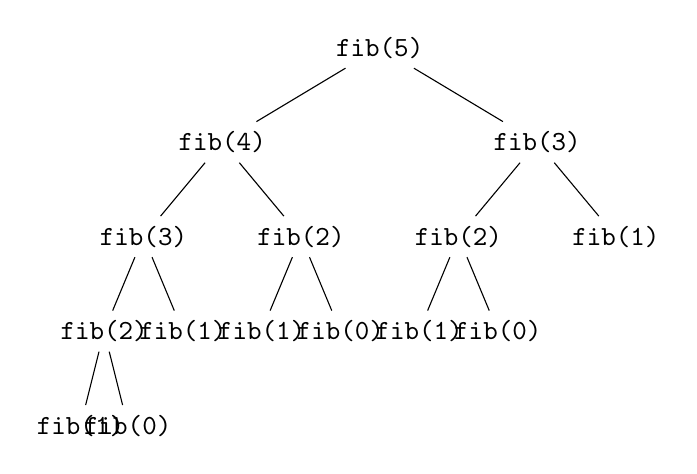
\begin{tikzpicture}[level distance=1.2cm,
                    level 1/.style={sibling distance=4cm},
                    level 2/.style={sibling distance=2cm},
                    level 3/.style={sibling distance=1cm},
                    level 4/.style={sibling distance=0.6cm}]
\node {\slate{fib(5)}}
    child {node {\slate{fib(4)}}
        child {node {\slate{fib(3)}}
            child {node {\slate{fib(2)}}
                child {node {\slate{fib(1)}}}
                child {node {\slate{fib(0)}}}
            }
            child {node {\slate{fib(1)}}}
        }
        child {node {\slate{fib(2)}}
            child {node {\slate{fib(1)}}}
            child {node {\slate{fib(0)}}}
        }
    }
    child {node {\slate{fib(3)}}
        child {node {\slate{fib(2)}}
            child {node {\slate{fib(1)}}}
            child {node {\slate{fib(0)}}}
        }
        child {node {\slate{fib(1)}}}
    };
\end{tikzpicture}
\caption{The tree-recursive process generated in computing \slate{fib(5)}.}
\label{fig:tree-recursive-fib}
\end{figure}

This procedure is instructive as a prototypical tree recursion, but it is a terrible way to compute Fibonacci numbers because it does so much redundant computation. Notice in Figure~\ref{fig:tree-recursive-fib} that the entire computation of \slate{fib(3)}---almost half the work---is duplicated. In fact, it is not hard to show that the number of times the procedure will compute \slate{fib(1)} or \slate{fib(0)} (the number of leaves in the above tree, in general) is precisely $\text{Fib}(n + 1)$. To get an idea of how bad this is, one can show that the value of $\text{Fib}(n)$ grows exponentially with $n$. More precisely (see Exercise 1.13), $\text{Fib}(n)$ is the closest integer to $\phi^n/\sqrt{5}$, where

$\phi = \frac{1 + \sqrt{5}}{2} \approx 1.6180$

is the golden ratio, which satisfies the equation

$\phi^2 = \phi + 1$.

Thus, the process uses a number of steps that grows exponentially with the input. On the other hand, the space required grows only linearly with the input, because we need keep track only of which nodes are above us in the tree at any point in the computation. In general, the number of steps required by a tree-recursive process will be proportional to the number of nodes in the tree, while the space required will be proportional to the maximum depth of the tree.

We can also formulate an iterative process for computing the Fibonacci numbers. The idea is to use a pair of integers $a$ and $b$, initialized to $\text{Fib}(1) = 1$ and $\text{Fib}(0) = 0$, and to repeatedly apply the simultaneous transformations

$a \leftarrow a + b$,
$b \leftarrow a$.

It is not hard to show that, after applying this transformation $n$ times, $a$ and $b$ will be equal, respectively, to $\text{Fib}(n + 1)$ and $\text{Fib}(n)$. Thus, we can compute Fibonacci numbers iteratively using the procedure

\begin{lstlisting}
def fib(n) = fib_iter(1, 0, n)

def fib_iter(a, b, count) =
    if count == 0 then
        b
    else
        fib_iter(a + b, a, count - 1)
\end{lstlisting}

This second method for computing $\text{Fib}(n)$ is a linear iteration. The difference in number of steps required by the two methods---one linear in $n$, one growing as fast as $\text{Fib}(n)$ itself---is enormous, even for small inputs.

One should not conclude from this that tree-recursive processes are useless. When we consider processes that operate on hierarchically structured data rather than numbers, we will find that tree recursion is a natural and powerful tool. But even in numerical operations, tree-recursive processes can be useful in helping us to understand and design programs. For instance, although the first \slate{fib} procedure is much less efficient than the second one, it is more straightforward, being little more than a translation into Slate of the definition of the Fibonacci sequence. To formulate the iterative algorithm required noticing that the computation could be recast as an iteration with three state variables.

\subsubsection{Example: Counting change}

It takes only a bit of cleverness to come up with the iterative Fibonacci algorithm. In contrast, consider the following problem: How many different ways can we make change of \$1.00, given half-dollars, quarters, dimes, nickels, and pennies? More generally, can we write a procedure to compute the number of ways to change any given amount of money?

This problem has a simple solution as a recursive procedure. Suppose we think of the types of coins available as arranged in some order. Then the following relation holds:

The number of ways to change amount $a$ using $n$ kinds of coins equals

\begin{itemize}
\item the number of ways to change amount $a$ using all but the first kind of coin, plus
\item the number of ways to change amount $a - d$ using all $n$ kinds of coins, where $d$ is the denomination of the first kind of coin.
\end{itemize}

To see why this is true, observe that the ways to make change can be divided into two groups: those that do not use any of the first kind of coin, and those that do. Therefore, the total number of ways to make change for some amount is equal to the number of ways to make change for the amount without using any of the first kind of coin, plus the number of ways to make change assuming that we do use the first kind of coin. But the latter number is equal to the number of ways to make change for the amount that remains after using a coin of the first kind.

Thus, we can recursively reduce the problem of changing a given amount to the problem of changing smaller amounts using fewer kinds of coins. Consider this reduction rule carefully, and convince yourself that we can use it to describe an algorithm if we specify the following degenerate cases:

\begin{itemize}
\item If $a$ is exactly 0, we should count that as 1 way to make change.
\item If $a$ is less than 0, we should count that as 0 ways to make change.
\item If $n$ is 0, we should count that as 0 ways to make change.
\end{itemize}

We can easily translate this description into a recursive procedure:

\begin{lstlisting}
def count_change(amount) = cc(amount, 5)

def cc(amount, kinds_of_coins) =
    if amount == 0 then
        1
    elif amount < 0 or kinds_of_coins == 0 then
        0
    else
        cc(amount, kinds_of_coins - 1) +
        cc(amount - first_denomination(kinds_of_coins), kinds_of_coins)

def first_denomination(kinds_of_coins) =
    if kinds_of_coins == 1 then 1
    elif kinds_of_coins == 2 then 5
    elif kinds_of_coins == 3 then 10
    elif kinds_of_coins == 4 then 25
    elif kinds_of_coins == 5 then 50
\end{lstlisting}

(The \slate{first_denomination} procedure takes as input the number of kinds of coins available and returns the denomination of the first kind. Here we are thinking of the coins as arranged in order from largest to smallest, but any order would do as well.) We can now answer our original question about changing a dollar:

\begin{lstlisting}
count_change(100)
\end{lstlisting}
\textit{292}

\slate{count_change} generates a tree-recursive process with redundancies similar to those in our first implementation of \slate{fib}. (It will take quite a while for that 292 to be computed.) On the other hand, it is not obvious how to design a better algorithm for computing the result, and we leave this problem as a challenge. The observation that a tree-recursive process may be highly inefficient but often easy to specify and understand has led people to propose that one could get the best of both worlds by designing a ``smart compiler'' that could transform tree-recursive procedures into more efficient procedures that compute the same result.

\begin{description}
\item[Exercise 1.11] A function $f$ is defined by the rule that

\begin{equation}
f(n) = \begin{cases}
n & \text{if } n < 3, \\
f(n - 1) + 2f(n - 2) + 3f(n - 3) & \text{if } n \geq 3.
\end{cases}
\end{equation}

Write a procedure that computes $f$ by means of a recursive process. Write a procedure that computes $f$ by means of an iterative process.

\item[Exercise 1.12] The following pattern of numbers is called Pascal's triangle.

\begin{verbatim}
    1
   1 1
  1 2 1
 1 3 3 1
1 4 6 4 1
   . . .
\end{verbatim}

The numbers at the edge of the triangle are all 1, and each number inside the triangle is the sum of the two numbers above it. Write a procedure that computes elements of Pascal's triangle by means of a recursive process.

\item[Exercise 1.13] Prove that $\text{Fib}(n)$ is the closest integer to $\phi^n/\sqrt{5}$, where $\phi = (1 + \sqrt{5})/2$. Hint: Let $\psi = (1 - \sqrt{5})/2$. Use induction and the definition of the Fibonacci numbers (see Section 1.2.2) to prove that $\text{Fib}(n) = (\phi^n - \psi^n)/\sqrt{5}$.
\end{description}

\subsection{Orders of Growth}

The previous examples illustrate that processes can differ considerably in the rates at which they consume computational resources. One convenient way to describe this difference is to use the notion of \emph{order of growth} to obtain a gross measure of the resources required by a process as the inputs become larger.

Let $n$ be a parameter that measures the size of the problem, and let $R(n)$ be the amount of resources the process requires for a problem of size $n$. In our previous examples we took $n$ to be the number for which the function is to be computed, but there are other possibilities. For instance, if our goal is to compute an approximation to the square root of a number, we might take $n$ to be the number of digits accuracy required. For matrix multiplication we might take $n$ to be the number of rows in the matrices. In general there are a number of properties of the problem with respect to which it will be desirable to analyze a given process. Similarly, $R(n)$ might measure the number of internal storage registers used, the number of elementary machine operations performed, and so on. In computers that do only a fixed number of operations at a time, the time required will be proportional to the number of elementary machine operations performed.

We say that $R(n)$ has order of growth $\Theta(f(n))$, written $R(n) = \Theta(f(n))$ (pronounced ``theta of $f(n)$''), if there are positive constants $k_1$ and $k_2$ independent of $n$ such that

$k_1 f(n) \leq R(n) \leq k_2 f(n)$

for any sufficiently large value of $n$. (In other words, for large $n$, the value $R(n)$ is sandwiched between $k_1 f(n)$ and $k_2 f(n)$.)

For instance, with the linear recursive process for computing factorial described in Section 1.2.1, the number of steps grows proportionally to the input $n$. Thus, the steps required for this process grows as $\Theta(n)$. We also saw that the space required grows as $\Theta(n)$. For the iterative factorial, the number of steps is still $\Theta(n)$ but the space is $\Theta(1)$---that is, constant. The tree-recursive Fibonacci computation requires $\Theta(\phi^n)$ steps and $\Theta(n)$ space, where $\phi$ is the golden ratio described in Section 1.2.2.

Orders of growth provide only a crude description of the behavior of a process. For example, a process requiring $n^2$ steps and a process requiring $1000n^2$ steps and a process requiring $3n^2 + 10n + 17$ steps all have $\Theta(n^2)$ order of growth. On the other hand, order of growth provides a useful indication of how we may expect the behavior of the process to change as we change the size of the problem. For a $\Theta(n)$ (linear) process, doubling the size will roughly double the amount of resources used. For an exponential process, each increment in problem size will multiply the resource utilization by a constant factor. In the remainder of Section 1.2 we will examine two algorithms whose order of growth is logarithmic, so that doubling the problem size increases the resource requirement by a constant amount.

\begin{description}
\item[Exercise 1.14] Draw the tree illustrating the process generated by the \slate{count_change} procedure of Section 1.2.2 in making change for 11 cents. What are the orders of growth of the space and number of steps used by this process as the amount to be changed increases?

\item[Exercise 1.15] The sine of an angle (specified in radians) can be computed by making use of the approximation $\sin x \approx x$ if $x$ is sufficiently small, and the trigonometric identity

$\sin x = 3 \sin \frac{x}{3} - 4 \sin^3 \frac{x}{3}$

to reduce the size of the argument of $\sin$. (For purposes of this exercise an angle is considered ``sufficiently small'' if its magnitude is not greater than 0.1 radians.) These ideas are incorporated in the following procedures:

\begin{lstlisting}
def cube(x) = x * x * x

def p(x) = 3 * x - 4 * cube(x)

def sine(angle) =
    if abs(angle) <= 0.1 then
        angle
    else
        p(sine(angle / 3.0))
\end{lstlisting}

\begin{enumerate}[label=\alph*.]
\item How many times is the procedure \slate{p} applied when \slate{sine(12.15)} is evaluated?
\item What is the order of growth in space and number of steps (as a function of $a$) used by the process generated by the \slate{sine} procedure when \slate{sine(a)} is evaluated?
\end{enumerate}
\end{description}

\subsection{Exponentiation}

Consider the problem of computing the exponential of a given number. We would like a procedure that takes as arguments a base $b$ and a positive integer exponent $n$ and computes $b^n$. One way to do this is via the recursive definition

\begin{align}
b^n &= b \cdot b^{n-1} \\
b^0 &= 1
\end{align}

which translates readily into the procedure

\begin{lstlisting}
def expt(b, n) =
    if n == 0 then
        1
    else
        b * expt(b, n - 1)
\end{lstlisting}

This is a linear recursive process, which requires $\Theta(n)$ steps and $\Theta(n)$ space. Just as with factorial, we can readily formulate an equivalent linear iteration:

\begin{lstlisting}
def expt(b, n) = expt_iter(b, n, 1)

def expt_iter(b, counter, product) =
    if counter == 0 then
        product
    else
        expt_iter(b, counter - 1, b * product)
\end{lstlisting}

This version requires $\Theta(n)$ steps and $\Theta(1)$ space.

We can compute exponentials in fewer steps by using successive squaring. For instance, rather than computing $b^8$ as

$b \cdot (b \cdot (b \cdot (b \cdot (b \cdot (b \cdot (b \cdot b))))))$

we can compute it using three multiplications:

\begin{align}
b^2 &= b \cdot b \\
b^4 &= b^2 \cdot b^2 \\
b^8 &= b^4 \cdot b^4
\end{align}

This method works fine for exponents that are powers of 2. We can also take advantage of successive squaring in computing exponentials in general if we use the rule

\begin{equation}
b^n = \begin{cases}
(b^{n/2})^2 & \text{if } n \text{ is even} \\
b \cdot b^{n-1} & \text{if } n \text{ is odd}
\end{cases}
\end{equation}

We can express this method as a procedure:

\begin{lstlisting}
def fast_expt(b, n) =
    if n == 0 then 1
    elif even(n) then square(fast_expt(b, n / 2))
    else b * fast_expt(b, n - 1)

def even(n) = (n % 2) == 0

def square(x) = x * x
\end{lstlisting}

The process evolved by \slate{fast_expt} grows logarithmically with $n$ in both space and number of steps. To see this, observe that computing $b^{2n}$ using \slate{fast_expt} requires only one more multiplication than computing $b^n$. The size of the exponent we can compute therefore doubles (approximately) with every new multiplication we are allowed. Thus, the number of multiplications required for an exponent of $n$ grows as $\Theta(\log n)$. The process has $\Theta(\log n)$ growth.

The difference between $\Theta(\log n)$ growth and $\Theta(n)$ growth becomes striking as $n$ becomes large. For example, \slate{fast_expt} for $n = 1000$ requires only 14 multiplications. It is also possible to use the idea of successive squaring to devise an iterative algorithm that computes exponentials with a logarithmic number of steps (see Exercise 1.16), although, as is often the case with iterative algorithms, this is not written down so straightforwardly as the recursive algorithm.

\begin{description}
\item[Exercise 1.16] Design a procedure that evolves an iterative exponentiation process that uses a logarithmic number of steps, as does \slate{fast_expt}. (Hint: Using the observation that $(b^{n/2})^2 = (b^2)^{n/2}$, keep, along with the exponent $n$ and the base $b$, an additional state variable $a$, and define the state transformation in such a way that the product $a b^n$ is unchanged from state to state. At the beginning of the process $a$ is taken to be 1, and the answer is given by the value of $a$ at the end of the process. In general, the technique of defining an \emph{invariant quantity} that remains unchanged from state to state is a powerful way to think about the design of iterative algorithms.)

\item[Exercise 1.17] The exponentiation algorithms in this section are based on performing exponentiation by means of repeated multiplication. In a similar way, one can perform integer multiplication by means of repeated addition. The following multiplication procedure (in which it is assumed that our language can only add, not multiply) is analogous to the \slate{expt} procedure:

\begin{lstlisting}
def mul(a, b) =
    if b == 0 then
        0
    else
        a + mul(a, b - 1)
\end{lstlisting}

This algorithm takes a number of steps that is linear in $b$. Now suppose we include, together with addition, operations \slate{double}, which doubles an integer, and \slate{halve}, which divides an (even) integer by 2. Using these, design a multiplication procedure analogous to \slate{fast_expt} that uses a logarithmic number of steps.

\item[Exercise 1.18] Using the results of Exercises 1.16 and 1.17, devise a procedure that generates an iterative process for multiplying two integers in terms of adding, doubling, and halving and uses a logarithmic number of steps.

\item[Exercise 1.19] There is a clever algorithm for computing the Fibonacci numbers in a logarithmic number of steps. Recall the transformation of the state variables $a$ and $b$ in the \slate{fib_iter} process of Section 1.2.2: $a \leftarrow a + b$ and $b \leftarrow a$. Call this transformation $T$, and observe that applying $T$ over and over again $n$ times, starting with 1 and 0, produces the pair $\text{Fib}(n + 1)$ and $\text{Fib}(n)$. In other words, the Fibonacci numbers are produced by applying $T^n$, the $n$th power of the transformation $T$, starting with the pair $(1,0)$. Now consider $T$ to be the special case of $p = 0$ and $q = 1$ in a family of transformations $T_{pq}$, where $T_{pq}$ transforms the pair $(a,b)$ according to $a \leftarrow bq + aq + ap$ and $b \leftarrow bp + aq$. Show that if we apply such a transformation $T_{pq}$ twice, the effect is the same as using a single transformation $T_{p'q'}$ of the same form, and compute $p'$ and $q'$ in terms of $p$ and $q$. This gives us an explicit way to square these transformations, which we can use to compute $T^n$ using successive squaring, as in the \slate{fast_expt} procedure. Put this all together to complete the following procedure, which runs in a logarithmic number of steps:

\begin{lstlisting}
def fib(n) = fib_iter(1, 0, 0, 1, n)

def fib_iter(a, b, p, q, count) =
    if count == 0 then
        b
    elif even(count) then
        fib_iter(a,
                 b,
                 ???,  \\ compute p'
                 ???,  \\ compute q'
                 count / 2)
    else
        fib_iter(b * q + a * q + a * p,
                 b * p + a * q,
                 p,
                 q,
                 count - 1)
\end{lstlisting}
\end{description}

\subsection{Greatest Common Divisors}

The greatest common divisor (GCD) of two integers $a$ and $b$ is defined to be the largest integer that divides both $a$ and $b$ with no remainder. For example, the GCD of 16 and 28 is 4. In Chapter 2, when we investigate how to implement rational-number arithmetic, we will need a procedure that computes the GCD of two integers. One way to find the GCD of two integers is to factor them and search for common factors, but there is a famous algorithm that is much more efficient.

The idea of the algorithm is based on the observation that, if $r$ is the remainder when $a$ is divided by $b$, then the common divisors of $a$ and $b$ are precisely the same as the common divisors of $b$ and $r$. Thus, we can use the equation

$\gcd(a,b) = \gcd(b,r)$

to successively reduce the problem of computing a GCD to the problem of computing the GCD of smaller and smaller pairs of integers. For example,

\begin{align}
\gcd(206,40) &= \gcd(40,6) \\
&= \gcd(6,4) \\
&= \gcd(4,2) \\
&= \gcd(2,0) \\
&= 2
\end{align}

reduces $\gcd(206,40)$ to $\gcd(2,0)$, which is 2. It is possible to show that starting with any two positive integers, this repeated reduction will always eventually produce a pair where the second number is 0. Then the GCD is the other number in the pair. This method for computing the GCD is known as Euclid's Algorithm.

It is easy to express Euclid's Algorithm as a procedure:

\begin{lstlisting}
def gcd(a, b) =
    if b == 0 then
        a
    else
        gcd(b, a % b)
\end{lstlisting}

This generates an iterative process, whose number of steps grows as the logarithm of the numbers involved.

The fact that the number of steps required by Euclid's Algorithm has logarithmic growth provides another example of the value of expressing programs as recursive procedures. Although the procedure is specified in terms of a recursive call to itself, the underlying process is actually iterative (see the discussion in Section 1.2.1). It is quite easy to verify this by noting that all the procedure does is transform the problem parameters according to a fixed rule. The number of steps required by Euclid's Algorithm to compute the GCD of two integers is proportional to the logarithm of the smaller of the two integers.

\begin{description}
\item[Exercise 1.20] The process that a procedure generates is of course dependent on the rules used by the interpreter. As an example, consider the iterative \slate{gcd} procedure given above. Suppose we were to interpret this procedure using normal-order evaluation, as discussed in Section 1.1.5. (The normal-order-evaluation rule is to evaluate the operator and operands and then apply the resulting procedure.) Using the substitution method (for normal order), illustrate the process generated in evaluating \slate{gcd(206, 40)} and indicate the \slate{remainder} operations that are actually performed. How many \slate{remainder} operations are actually performed in the normal-order evaluation of \slate{gcd(206, 40)}? In the applicative-order evaluation?
\end{description}

\subsection{Example: Testing for Primality}

This section describes two methods for checking the primality of an integer $n$, one with order of growth $\Theta(\sqrt{n})$, and a ``probabilistic'' algorithm with order of growth $\Theta(\log n)$. The exercises at the end of this section suggest programming projects based on these algorithms.

\subsubsection{Searching for divisors}

Since ancient times, mathematicians have been fascinated by problems concerning prime numbers, and many people have worked on the problem of determining ways to test if numbers are prime. One way to test if a number is prime is to find the number's divisors. The following program finds the smallest integral divisor (greater than 1) of a given number $n$. It does this in a straightforward way, by testing $n$ for divisibility by successive integers starting with 2.

\begin{lstlisting}
def smallest_divisor(n) = find_divisor(n, 2)

def find_divisor(n, test_divisor) =
    if square(test_divisor) > n then
        n
    elif divides(test_divisor, n) then
        test_divisor
    else
        find_divisor(n, test_divisor + 1)

def divides(a, b) = (b % a) == 0
\end{lstlisting}

We can test whether a number is prime as follows: $n$ is prime if and only if $n$ is its own smallest divisor.

\begin{lstlisting}
def prime(n) = n == smallest_divisor(n)
\end{lstlisting}

The end test for \slate{find_divisor} is based on the fact that if $n$ is not prime it must have a divisor less than or equal to $\sqrt{n}$. This means that the algorithm need only test divisors between 1 and $\sqrt{n}$. Consequently, the number of steps required to identify $n$ as prime will have order of growth $\Theta(\sqrt{n})$.

\subsubsection{The Fermat test}

The $\Theta(\log n)$ primality test is based on a result from number theory known as Fermat's Little Theorem.

\textbf{Fermat's Little Theorem:} If $n$ is a prime number and $a$ is any positive integer less than $n$, then $a$ raised to the $n$th power is congruent to $a$ modulo $n$.

(Two numbers are said to be \emph{congruent modulo} $n$ if they both have the same remainder when divided by $n$. The remainder of a number $a$ when divided by $n$ is also referred to as the \emph{remainder of $a$ modulo $n$}, or simply as \emph{$a$ modulo $n$}.)

If $n$ is not prime, then, in general, most of the numbers $a < n$ will not satisfy the above relation. This leads to the following algorithm for testing primality: Given a number $n$, pick a random number $a < n$ and compute the remainder of $a^n$ modulo $n$. If the result is not equal to $a$, then $n$ is certainly not prime. If it is $a$, then chances are good that $n$ is prime. Now pick another random number $a$ and test it with the same method. If it also satisfies the equation, then we can be even more confident that $n$ is prime. By trying more and more values of $a$, we can increase our confidence in the result. This algorithm is known as the Fermat test.

To implement the Fermat test, we need a procedure that computes the exponential of a number modulo another number:

\begin{lstlisting}
def expmod(base, exp, m) =
    if exp == 0 then
        1
    elif even(exp) then
        square(expmod(base, exp / 2, m)) % m
    else
        (base * expmod(base, exp - 1, m)) % m
\end{lstlisting}

This is very similar to the \slate{fast_expt} procedure of Section 1.2.4. It uses successive squaring, so that the number of steps grows logarithmically with the exponent.

The Fermat test is performed by choosing at random a number $a$ between 1 and $n - 1$ inclusive and checking whether the remainder modulo $n$ of the $n$th power of $a$ is equal to $a$. The random number $a$ is chosen using the procedure \slate{random}, which we assume is included as a primitive in Slate. \slate{random} returns a nonnegative integer less than its integer input. Hence, to obtain a random number between 1 and $n - 1$, we call \slate{random(n - 1)} and add 1:

\begin{lstlisting}
def fermat_test(n) =
    def try_it(a) = (expmod(a, n, n) == a)
    try_it(1 + random(n - 1))
\end{lstlisting}

The following procedure runs the test a given number of times, as specified by a parameter. Its value is true if the test succeeds every time, and false otherwise.

\begin{lstlisting}
def fast_prime(n, times) =
    if times == 0 then
        true
    elif fermat_test(n) then
        fast_prime(n, times - 1)
    else
        false
\end{lstlisting}

\subsubsection{Probabilistic methods}

The Fermat test differs in character from most familiar algorithms, in which one computes an answer that is guaranteed to be correct. Here, the answer obtained is only probably correct. More precisely, if $n$ ever fails the Fermat test, we can be certain that $n$ is not prime. But the fact that $n$ passes the test, while an extremely strong indication, is still not a guarantee that $n$ is prime. What we would like to say is that for any number $n$, if we perform the test enough times and find that $n$ always passes the test, then the probability of error in our primality test can be made as small as we like.

Unfortunately, this assertion is not quite correct. There do exist numbers that fool the Fermat test: numbers $n$ that are not prime and yet have the property that $a^n$ is congruent to $a$ modulo $n$ for all integers $a < n$. Such numbers are extremely rare, so the Fermat test is quite reliable in practice. There are variants of the Fermat test that cannot be fooled. In these tests, as with the Fermat method, one tests the primality of an integer $n$ by choosing a random integer $a < n$ and checking some condition (easy to compute) involving $a$ and $n$. The difference is that these tests can prove that an integer is not prime without being subject to the error of false testimony to primality. (See Exercise 1.28.)

On the other hand, in contrast to algorithms whose results are either correct or incorrect, probabilistic algorithms can be highly useful in some applications. A prime example is the use of probabilistic primality testing in implementing a code-breaking system based on the RSA cryptographic algorithm. Numbers of several hundred digits are routinely tested for primality using probabilistic methods and then used as keys for RSA. The probabilities of error in such applications can be estimated, and can be made smaller than the probability of the most unlikely physical events (such as cosmic rays corrupting a computer memory) and well below any reasonable threshold for practical use.

\begin{description}
\item[Exercise 1.21] Use the \slate{smallest_divisor} procedure to find the smallest divisor of each of the following numbers: 199, 1999, 19999.

\item[Exercise 1.22] Most Slate implementations include a primitive called \slate{runtime} that returns an integer that specifies the amount of time the system has been running (measured, for example, in microseconds). The following \slate{timed_prime_test} procedure, when called with an integer $n$, prints $n$ and checks to see if $n$ is prime. If $n$ is prime, the procedure prints three asterisks followed by the amount of time used in performing the test.

\begin{lstlisting}
def timed_prime_test(n) =
    newline()
    display(n)
    start_prime_test(n, runtime())

def start_prime_test(n, start_time) =
    if prime(n) then
        report_prime(runtime() - start_time)

def report_prime(elapsed_time) =
    display(" *** ")
    display(elapsed_time)
\end{lstlisting}

Using this procedure, write a procedure \slate{search_for_primes} that checks the primality of consecutive odd integers in a specified range. Use your procedure to find the three smallest primes larger than 1000; larger than 10,000; larger than 100,000; larger than 1,000,000. Note the time needed to test each prime. Since the testing algorithm has order of growth $\Theta(\sqrt{n})$, you should expect that testing for primes around 10,000 should take about $\sqrt{10}$ times as long as testing for primes around 1000. Do your timing data bear this out? How well do the data for 100,000 and 1,000,000 support the $\Theta(\sqrt{n})$ prediction? Is your result compatible with the notion that programs on your machine run in time proportional to the number of steps required for the computation?

\item[Exercise 1.23] The \slate{smallest_divisor} procedure shown at the start of this section does lots of needless testing: After it checks to see if the number is divisible by 2 there is no point in checking to see if it is divisible by any larger even number. This suggests that the values used for \slate{test_divisor} should not be 2, 3, 4, 5, 6, \ldots, but rather 2, 3, 5, 7, 9, \ldots. To implement this change, define a procedure \slate{next} that returns 3 if its input is equal to 2 and otherwise returns its input plus 2. Modify the \slate{smallest_divisor} procedure to use \slate{(next test_divisor)} instead of \slate{(test_divisor + 1)}. With \slate{timed_prime_test} incorporating this modified version of \slate{smallest_divisor}, run the test for each of the 12 primes found in Exercise 1.22. Since this modification halves the number of test steps, you should expect it to run about twice as fast. Is this expectation confirmed? If not, what is the observed ratio of the speeds of the two algorithms, and how do you explain the fact that it is different from 2?

\item[Exercise 1.24] Modify the \slate{timed_prime_test} procedure of Exercise 1.22 to use \slate{fast_prime} (the Fermat method) instead of \slate{prime}, and test each of the 12 primes you found in that exercise. Since the Fermat test has $\Theta(\log n)$ growth, how would you expect the time to test primes near 1,000,000 to compare with the time needed to test primes near 1000? Do your data bear this out? Can you explain any discrepancy you find?

\item[Exercise 1.25] Alyssa P. Hacker complains that we went to a lot of extra work in writing \slate{expmod}. After all, she says, since we already know how to compute exponentials, we could have simply written

\begin{lstlisting}
def expmod(base, exp, m) = (fast_expt(base, exp)) % m
\end{lstlisting}

Is she correct? Would this procedure serve as well for our fast prime tester? Explain.

\item[Exercise 1.26] Louis Reasoner is having great difficulty doing Exercise 1.24. His \slate{fast_prime} test seems to run more slowly than his \slate{prime} test. Louis calls his friend Eva Lu Ator over to help. When they examine Louis's code, they find that he has rewritten the \slate{expmod} procedure to use an explicit multiplication, rather than calling \slate{square}:

\begin{lstlisting}
def expmod(base, exp, m) =
    if exp == 0 then
        1
    elif even(exp) then
        (expmod(base, exp / 2, m) * expmod(base, exp / 2, m)) % m
    else
        (base * expmod(base, exp - 1, m)) % m
\end{lstlisting}

``I don't see what difference that could make,'' says Louis. ``I do.'' says Eva. ``By writing the procedure like that, you have transformed the $\Theta(\log n)$ process into a $\Theta(n)$ process.'' Explain.

\item[Exercise 1.27] Demonstrate that the Carmichael numbers---561, 1105, 1729, 2465, 2821, and 6601---really do fool the Fermat test. That is, write a procedure that takes an integer $n$ and tests whether $a^n$ is congruent to $a$ modulo $n$ for every $a < n$, and try your procedure on the given Carmichael numbers.

\item[Exercise 1.28] One variant of the Fermat test that cannot be fooled is called the \emph{Miller-Rabin test} (Miller 1976; Rabin 1980). This starts from an alternate form of Fermat's Little Theorem, which states that if $n$ is a prime number and $a$ is any positive integer less than $n$, then $a$ raised to the $(n - 1)$st power is congruent to 1 modulo $n$. To test the primality of a number $n$ by the Miller-Rabin test, we pick a random number $a < n$ and raise $a$ to the $(n - 1)$st power modulo $n$ using the \slate{expmod} procedure. However, whenever we perform the squaring step in \slate{expmod}, we check to see if we have discovered a ``nontrivial square root of 1 modulo $n$,'' that is, a number not equal to 1 or $n - 1$ whose square is equal to 1 modulo $n$. It is possible to prove that if such a nontrivial square root of 1 exists, then $n$ is not prime. It is also possible to prove that if $n$ is an odd number that is not prime, then, for at least half the numbers $a < n$, computing $a^{n-1}$ in this way will reveal a nontrivial square root of 1 modulo $n$. (This is why the Miller-Rabin test cannot be fooled.) Modify the \slate{expmod} procedure to signal if it discovers a nontrivial square root of 1, and use this to implement the Miller-Rabin test with a procedure analogous to \slate{fermat_test}. Check your procedure by testing it on some known primes and non-primes. Hint: One convenient way to make \slate{expmod} signal is to have it return 0.
\end{description}

% Section 1.3: Formulating Abstractions with Higher-Order Procedures
\section{Formulating Abstractions with Higher-Order Procedures}

We have seen that procedures are, in effect, abstractions that describe compound operations on numbers independent of the particular numbers. For example, when we

\begin{lstlisting}[style=slate]
def cube(x) = x * x * x
\end{lstlisting}

we are not talking about the cube of a particular number, but rather about a method for obtaining the cube of any number. Of course we could get along without ever defining this procedure, by always writing expressions such as

\begin{lstlisting}[style=slate]
3 * 3 * 3
x * x * x
y * y * y
\end{lstlisting}

and never mentioning \slate{cube} explicitly. This would place us at a serious disadvantage, forcing us to work always at the level of the particular operations that happen to be primitives in the language (multiplication, in this case) rather than in terms of higher-level operations. Our programs would be able to compute cubes, but our language would lack the ability to express the concept of cubing. One of the things we should demand from a powerful programming language is the ability to build abstractions by assigning names to common patterns and then to work in terms of the abstractions directly. Procedures provide this ability. This is why all but the most primitive programming languages include mechanisms for defining procedures.

Yet even in numerical processing we will be severely limited in our ability to create abstractions if we are restricted to procedures whose parameters must be numbers. Often the same programming pattern will be used with a number of different procedures. To express such patterns as concepts, we will need to construct procedures that can accept procedures as arguments or return procedures as values. Procedures that manipulate procedures are called \emph{higher-order procedures}. This section shows how higher-order procedures can serve as powerful abstraction mechanisms, vastly increasing the expressive power of our language.

\subsection{Procedures as Arguments}

Consider the following three procedures. The first computes the sum of the integers from \slate{a} through \slate{b}:

\begin{lstlisting}[style=slate]
def sum_integers(a, b) =
    if a > b then 0
    else a + sum_integers(a + 1, b)
\end{lstlisting}

The second computes the sum of the cubes of the integers in the given range:

\begin{lstlisting}[style=slate]
def sum_cubes(a, b) =
    if a > b then 0
    else cube(a) + sum_cubes(a + 1, b)
\end{lstlisting}

The third computes the sum of a sequence of terms in the series
\[
\frac{1}{1 \cdot 3} + \frac{1}{5 \cdot 7} + \frac{1}{9 \cdot 11} + \cdots,
\]
which converges to $\pi/8$ (very slowly):\footnote{This series, usually written in the equivalent form $\frac{\pi}{4} = 1 - \frac{1}{3} + \frac{1}{5} - \frac{1}{7} + \cdots$, is due to Leibniz. We'll see how to use this as the basis for some fancy numerical tricks in Section 3.5.3.}

\begin{lstlisting}[style=slate]
def pi_sum(a, b) =
    if a > b then 0
    else (1.0 / (a * (a + 2))) + pi_sum(a + 4, b)
\end{lstlisting}

These three procedures clearly share a common underlying pattern. They are for the most part identical, differing only in the name of the procedure, the function of \slate{a} used to compute the term to be added, and the function that provides the next value of \slate{a}. We could generate each of the procedures by filling in slots in the same template:

\begin{lstlisting}[style=plain]
def $\langle$name$\rangle$(a, b) =
    if a > b then 0
    else $\langle$term$\rangle$(a) + $\langle$name$\rangle$($\langle$next$\rangle$(a), b)
\end{lstlisting}

The presence of such a common pattern is strong evidence that there is a useful abstraction waiting to be brought to the surface. Indeed, mathematicians long ago identified the abstraction of \emph{summation of a series} and invented ``sigma notation,'' for example
\[
\sum_{n=a}^{b} f(n) = f(a) + \cdots + f(b),
\]
to express this concept. The power of sigma notation is that it allows mathematicians to deal with the concept of summation itself rather than only with particular sums---for example, to formulate general results about sums that are independent of the particular series being summed.

Similarly, as program designers, we would like our language to be powerful enough so that we can write a procedure that expresses the concept of summation itself rather than only procedures that compute particular sums. We can do so readily in our procedural language by taking the common template shown above and transforming the ``slots'' into formal parameters:

\begin{lstlisting}[style=slate]
def sum(term, a, next, b) =
    if a > b then 0
    else term(a) + sum(term, next(a), next, b)
\end{lstlisting}

Notice that \slate{sum} takes as its arguments the lower and upper bounds \slate{a} and \slate{b} together with the procedures \slate{term} and \slate{next}. We can use \slate{sum} just as we would any procedure. For example, we can use it (along with a procedure \slate{inc} that increments its argument by 1) to define \slate{sum_cubes}:

\begin{lstlisting}[style=slate]
def inc(n) = n + 1

def sum_cubes(a, b) = sum(cube, a, inc, b)
\end{lstlisting}

Using this, we can compute the sum of the cubes of the integers from 1 to 10:

\begin{lstlisting}[style=slate]
sum_cubes(1, 10)
\end{lstlisting}
\begin{verbatim}
3025
\end{verbatim}

With the aid of an identity procedure to compute the term, we can define \slate{sum_integers} in terms of \slate{sum}:

\begin{lstlisting}[style=slate]
def identity(x) = x

def sum_integers(a, b) = sum(identity, a, inc, b)
\end{lstlisting}

Then we can add up the integers from 1 to 10:

\begin{lstlisting}[style=slate]
sum_integers(1, 10)
\end{lstlisting}
\begin{verbatim}
55
\end{verbatim}

We can also define \slate{pi_sum} in the same way:\footnote{Notice that we have used block structure (Section 1.1.8) to embed the definitions of \slate{pi_next} and \slate{pi_term} within \slate{pi_sum}, since these procedures are unlikely to be useful for any other purpose. We will see how to get rid of them altogether in Section 1.3.2.}

\begin{lstlisting}[style=slate]
def pi_sum(a, b) =
    def pi_term(x) = 1.0 / (x * (x + 2))
    def pi_next(x) = x + 4
    sum(pi_term, a, pi_next, b)
\end{lstlisting}

Using these procedures, we can compute an approximation to $\pi$:

\begin{lstlisting}[style=slate]
8 * pi_sum(1, 1000)
\end{lstlisting}
\begin{verbatim}
3.139592655589783
\end{verbatim}

Once we have \slate{sum}, we can use it as a building block in formulating further concepts. For instance, the definite integral of a function $f$ between the limits $a$ and $b$ can be approximated numerically using the formula
\[
\int_a^b f = \left[ f\left(a + \frac{dx}{2}\right) + f\left(a + dx + \frac{dx}{2}\right) + f\left(a + 2dx + \frac{dx}{2}\right) + \cdots \right] dx
\]
for small values of $dx$. We can express this directly as a procedure:

\begin{lstlisting}[style=slate]
def integral(f, a, b, dx) =
    def add_dx(x) = x + dx
    sum(f, a + (dx / 2.0), add_dx, b) * dx
\end{lstlisting}

\begin{lstlisting}[style=slate]
integral(cube, 0, 1, 0.01)
\end{lstlisting}
\begin{verbatim}
0.24998750000000042
\end{verbatim}

\begin{lstlisting}[style=slate]
integral(cube, 0, 1, 0.001)
\end{lstlisting}
\begin{verbatim}
0.249999875000001
\end{verbatim}

(The exact value of the integral of cube between 0 and 1 is 1/4.)

\textbf{Exercise 1.29:} Simpson's Rule is a more accurate method of numerical integration than the method illustrated above. Using Simpson's Rule, the integral of a function $f$ between $a$ and $b$ is approximated as
\[
\frac{h}{3}(y_0 + 4y_1 + 2y_2 + 4y_3 + 2y_4 + \cdots + 2y_{n-2} + 4y_{n-1} + y_n),
\]
where $h = (b-a)/n$, for some even integer $n$, and $y_k = f(a + kh)$. (Increasing $n$ increases the accuracy of the approximation.) Define a procedure that takes as arguments $f$, $a$, $b$, and $n$ and returns the value of the integral, computed using Simpson's Rule. Use your procedure to integrate \slate{cube} between 0 and 1 (with $n = 100$ and $n = 1000$), and compare the results to those of the \slate{integral} procedure shown above.

\textbf{Exercise 1.30:} The \slate{sum} procedure above generates a linear recursion. The procedure can be rewritten so that the sum is performed iteratively. Show how to do this by filling in the missing expressions in the following definition:

\begin{lstlisting}[style=plain]
def sum(term, a, next, b) =
    def iter(a, result) =
        if $\langle$??$\rangle$ then $\langle$??$\rangle$
        else iter($\langle$??$\rangle$, $\langle$??$\rangle$)
    iter($\langle$??$\rangle$, $\langle$??$\rangle$)
\end{lstlisting}

\textbf{Exercise 1.31:}
\begin{enumerate}
\item The \slate{sum} procedure is only the simplest of a vast number of similar abstractions that can be captured as higher-order procedures.\footnote{The intent of Exercises 1.31 through 1.33 is to demonstrate the expressive power that is attained by using an appropriate abstraction to consolidate many seemingly disparate operations. However, though accumulation and filtering are elegant ideas, our hands are somewhat tied in using them at this point since we do not yet have data structures to provide suitable means of combination for these abstractions. We will return to these ideas in Section 2.2.3 when we show how to use sequences as interfaces for combining filters and accumulators to build even more powerful abstractions. We will see there how these methods really come into their own as a powerful and elegant approach to designing programs.} Write an analogous procedure called \slate{product} that returns the product of the values of a function at points over a given range. Show how to define \slate{factorial} in terms of \slate{product}. Also use \slate{product} to compute approximations to $\pi$ using the formula\footnote{This formula was discovered by the seventeenth-century English mathematician John Wallis.}
\[
\frac{\pi}{4} = \frac{2 \cdot 4 \cdot 4 \cdot 6 \cdot 6 \cdot 8 \cdots}{3 \cdot 3 \cdot 5 \cdot 5 \cdot 7 \cdot 7 \cdots}.
\]

\item If your \slate{product} procedure generates a recursive process, write one that generates an iterative process. If it generates an iterative process, write one that generates a recursive process.
\end{enumerate}

\textbf{Exercise 1.32:}
\begin{enumerate}
\item Show that \slate{sum} and \slate{product} (Exercise 1.31) are both special cases of a still more general notion called \slate{accumulate} that combines a collection of terms, using some general accumulation function:

\begin{lstlisting}[style=slate]
accumulate(combiner, null_value, term, a, next, b)
\end{lstlisting}

\slate{accumulate} takes as arguments the same \slate{term} and range specifications as \slate{sum} and \slate{product}, together with a \slate{combiner} procedure (of two arguments) that specifies how the current term is to be combined with the accumulation of the preceding terms and a \slate{null_value} that specifies what base value to use when the terms run out. Write \slate{accumulate} and show how \slate{sum} and \slate{product} can both be defined as simple calls to \slate{accumulate}.

\item If your \slate{accumulate} procedure generates a recursive process, write one that generates an iterative process. If it generates an iterative process, write one that generates a recursive process.
\end{enumerate}

\textbf{Exercise 1.33:} You can obtain an even more general version of \slate{accumulate} (Exercise 1.32) by introducing the notion of a \emph{filter} on the terms to be combined. That is, combine only those terms derived from values in the range that satisfy a specified condition. The resulting \slate{filtered_accumulate} abstraction takes the same arguments as \slate{accumulate}, together with an additional predicate of one argument that specifies the filter. Write \slate{filtered_accumulate} as a procedure. Show how to express the following using \slate{filtered_accumulate}:

\begin{enumerate}
\item the sum of the squares of the prime numbers in the interval $a$ to $b$ (assuming that you have a \slate{prime?} predicate already written)

\item the product of all the positive integers less than $n$ that are relatively prime to $n$ (i.e., all positive integers $i < n$ such that $\gcd(i,n) = 1$).
\end{enumerate}

\subsection{Constructing Procedures Using Anonymous Functions}

In using \slate{sum} as in Section 1.3.1, it seems terribly awkward to have to define trivial procedures such as \slate{pi_term} and \slate{pi_next} just so we can use them as arguments to our higher-order procedure. Rather than define \slate{pi_next} and \slate{pi_term}, it would be more convenient to have a way to directly specify ``the procedure that returns its input incremented by 4'' and ``the procedure that returns the reciprocal of its input times its input plus 2.'' We can do this by using Slate's anonymous function syntax.

In Slate, we can describe what we want as

\begin{lstlisting}[style=slate]
x -> x + 4
\end{lstlisting}

and

\begin{lstlisting}[style=slate]
x -> 1.0 / (x * (x + 2))
\end{lstlisting}

Then our \slate{pi_sum} procedure can be expressed without defining any auxiliary procedures as

\begin{lstlisting}[style=slate]
def pi_sum(a, b) =
    sum(x -> 1.0 / (x * (x + 2)), 
        a,
        x -> x + 4,
        b)
\end{lstlisting}

Again using anonymous functions, we can write the \slate{integral} procedure without having to define the auxiliary procedure \slate{add_dx}:

\begin{lstlisting}[style=slate]
def integral(f, a, b, dx) =
    sum(f, a + (dx / 2.0), x -> x + dx, b) * dx
\end{lstlisting}

In general, anonymous functions are used to create procedures in the same way as \slate{def}, except that no name is specified for the procedure:

\begin{lstlisting}[style=plain]
def($\langle$formal-parameters$\rangle$) = $\langle$body$\rangle$
\end{lstlisting}

The resulting procedure is just as much a procedure as one that is created using \slate{def}. The only difference is that it has not been associated with any name in the environment. In fact,

\begin{lstlisting}[style=slate]
def plus4(x) = x + 4
\end{lstlisting}

is equivalent to

\begin{lstlisting}[style=slate]
val plus4 = x -> x + 4
\end{lstlisting}

We can read an anonymous function expression as follows:

\begin{lstlisting}[style=slate]
x -> x + 4
\end{lstlisting}

means ``the function of an argument \slate{x} that adds \slate{x} and 4.''

Like any expression that has a procedure as its value, an anonymous function expression can be used as the operator in a combination such as

\begin{lstlisting}[style=slate]
((x, y, z) -> x + y + (z * z))(1, 2, 3)
\end{lstlisting}
\begin{verbatim}
12
\end{verbatim}

or, more generally, in any context where we would normally use a procedure name.

\subsubsection{Using \texttt{let} to create local variables}

Another use of anonymous functions is in creating local variables. We often need local variables in our procedures other than those that have been bound as formal parameters. For example, suppose we wish to compute the function

\[
f(x, y) = x(1 + xy)^2 + y(1 - y) + (1 + xy)(1 - y),
\]

which we could also express as

\begin{align}
a &= 1 + xy, \\
b &= 1 - y, \\
f(x, y) &= xa^2 + yb + ab.
\end{align}

In writing a procedure to compute $f$, we would like to include as local variables not only \slate{x} and \slate{y} but also the names of intermediate quantities like \slate{a} and \slate{b}. One way to accomplish this is to use an auxiliary procedure to bind the local variables:

\begin{lstlisting}[style=slate]
def f(x, y) =
    def f_helper(a, b) =
        x * (a * a) + y * b + a * b
    f_helper(1 + x * y, 1 - y)
\end{lstlisting}

Of course, we could use an anonymous function to specify an anonymous procedure for binding our local variables. The body of \slate{f} then becomes a single call to that procedure:

\begin{lstlisting}[style=slate]
def f(x, y) =
    ((a, b) -> x * (a * a) + y * b + a * b)(1 + x * y, 1 - y)
\end{lstlisting}

This construct is so useful that Slate provides a special syntax called \texttt{let} to make its use more convenient. Using \texttt{let}, the \slate{f} procedure could be written as

\begin{lstlisting}[style=slate]
def f(x, y) =
    let a = 1 + x * y
        b = 1 - y
    in
        x * (a * a) + y * b + a * b
\end{lstlisting}

The general form of a \texttt{let} expression is

\begin{lstlisting}[style=plain]
let $\langle$var1$\rangle$ = $\langle$exp1$\rangle$
    $\langle$var2$\rangle$ = $\langle$exp2$\rangle$
    ...
    $\langle$varn$\rangle$ = $\langle$expn$\rangle$
in $\langle$body$\rangle$
\end{lstlisting}

which can be thought of as saying

\begin{quote}
let \texttt{$\langle$var1$\rangle$} have the value \texttt{$\langle$exp1$\rangle$} and\\
\texttt{$\langle$var2$\rangle$} have the value \texttt{$\langle$exp2$\rangle$} and\\
\ldots\\
\texttt{$\langle$varn$\rangle$} have the value \texttt{$\langle$expn$\rangle$}\\
in \texttt{$\langle$body$\rangle$}
\end{quote}

The first part of the \texttt{let} expression is a list of name-expression pairs. When the \texttt{let} is evaluated, each name is associated with the value of the corresponding expression. The body of the \texttt{let} is evaluated with these names bound as local variables. The way this happens is that the \texttt{let} expression is interpreted as an alternate syntax for

\begin{lstlisting}[style=plain]
(def($\langle$var1$\rangle$, ..., $\langle$varn$\rangle$) = $\langle$body$\rangle$)($\langle$exp1$\rangle$, ..., $\langle$expn$\rangle$)
\end{lstlisting}

No new mechanism is required in the interpreter in order to provide local variables. A \texttt{let} expression is simply syntactic sugar for the underlying anonymous function application.

We can see from this equivalence that the scope of a variable specified by a \texttt{let} expression is the body of the \texttt{let}. This implies that:

\begin{itemize}
\item \texttt{let} allows one to bind variables as locally as possible to where they are to be used. For example, if the value of \slate{x} is 5, the value of the expression

\begin{lstlisting}[style=slate]
let x = 3 in x * (x + 10) + x
\end{lstlisting}

is 38. Here, the \slate{x} in the body of the \texttt{let} is 3, so the value of the \texttt{let} expression is 33. On the other hand, the \slate{x} that is the second argument to the outermost \texttt{+} is still 5.

\item The variables' values are computed outside the \texttt{let}. This matters when the expressions that provide the values for the local variables depend upon variables having the same names as the local variables themselves. For example, if the value of \slate{x} is 2, the expression

\begin{lstlisting}[style=slate]
let x = 3
    y = x + 2
in x * y
\end{lstlisting}

will have the value 12 because, inside the body of the \texttt{let}, \slate{x} will be 3 and \slate{y} will be 4 (which is the outer \slate{x} plus 2).
\end{itemize}

Sometimes we can use internal definitions to get the same effect as with \texttt{let}. For example, we could have defined the procedure \slate{f} above as

\begin{lstlisting}[style=slate]
def f(x, y) =
    val a = 1 + x * y
    val b = 1 - y
    x * (a * a) + y * b + a * b
\end{lstlisting}

We prefer, however, to use \texttt{let} in situations like this and to use internal \texttt{def} only for internal procedures.

\textbf{Exercise 1.34:} Suppose we define the procedure

\begin{lstlisting}[style=slate]
def f(g) = g(2)
\end{lstlisting}

Then we have

\begin{lstlisting}[style=slate]
f(square)
\end{lstlisting}
\begin{verbatim}
4
\end{verbatim}

\begin{lstlisting}[style=slate]
f(z -> z * (z + 1))
\end{lstlisting}
\begin{verbatim}
6
\end{verbatim}

What happens if we (perversely) ask the interpreter to evaluate the combination \slate{f(f)}? Explain.

\subsection{Procedures as General Methods}

We introduced compound procedures in Section 1.1.4 as a mechanism for abstracting patterns of numerical operations so as to make them independent of the particular numbers involved. With higher-order procedures, such as the \slate{integral} procedure of Section 1.3.1, we began to see a more powerful kind of abstraction: procedures used to express general methods of computation, independent of the particular functions involved. In this section we discuss two more elaborate examples---general methods for finding zeros and fixed points of functions---and show how these methods can be expressed directly as procedures.

\subsubsection{Finding roots of equations by the half-interval method}

The \emph{half-interval method} is a simple but powerful technique for finding roots of an equation $f(x) = 0$, where $f$ is a continuous function. The idea is that, if we are given points $a$ and $b$ such that $f(a) < 0 < f(b)$, then $f$ must have at least one zero between $a$ and $b$. To locate a zero, let $x$ be the average of $a$ and $b$, and compute $f(x)$. If $f(x) > 0$, then $f$ must have a zero between $a$ and $x$. If $f(x) < 0$, then $f$ must have a zero between $x$ and $b$. Continuing in this way, we can identify smaller and smaller intervals on which $f$ must have a zero. When we reach a point where the interval is small enough, the process stops. Since the interval of uncertainty is reduced by half at each step of the process, the number of steps required grows as $\Theta(\log(L/T))$, where $L$ is the length of the original interval and $T$ is the error tolerance (that is, the size of the interval we will consider ``small enough''). Here is a procedure that implements this strategy:

\begin{lstlisting}[style=slate]
def search(f, neg_point, pos_point) =
    val midpoint = average(neg_point, pos_point)
    if close_enough(neg_point, pos_point) then midpoint
    else
        val test_value = f(midpoint)
        if test_value > 0 then
            search(f, neg_point, midpoint)
        elif test_value < 0 then
            search(f, midpoint, pos_point)
        else
            midpoint
\end{lstlisting}

We assume that we are initially given the function \slate{f} together with points at which its values are negative and positive. We first compute the midpoint of the two given points. Next we check to see if the given interval is small enough, and if so we simply return the midpoint as our answer. Otherwise, we compute as a test value the value of \slate{f} at the midpoint. If the test value is positive, then we continue the process with a new interval running from the original negative point to the midpoint. If the test value is negative, we continue with the interval from the midpoint to the positive point. Finally, there is the possibility that the test value is 0, in which case the midpoint is itself the root we are searching for.

To test whether the endpoints are ``close enough'' we can use a procedure similar to the one used in Section 1.1.7 for computing square roots:\footnote{We have used 0.001 as a representative ``small'' number to indicate a tolerance for the acceptable error in a calculation. The appropriate tolerance for a real calculation depends upon the problem to be solved and the limitations of the computer and the algorithm. This is often a very subtle consideration, requiring help from a numerical analyst or some other kind of magician.}

\begin{lstlisting}[style=slate]
def close_enough(x, y) = abs(x - y) < 0.001
\end{lstlisting}

\slate{search} is awkward to use directly, because we can accidentally give it points at which \slate{f}'s values do not have the required sign, in which case we get a wrong answer. Instead we will use \slate{search} via the following procedure, which checks to see which of the endpoints has a negative function value and which has a positive value, and calls the \slate{search} procedure accordingly. If the function has the same sign on the two given points, the half-interval method cannot be used, in which case the procedure signals an error.\footnote{This can be accomplished using \slate{error}, which takes as arguments a number of items that are printed as error messages.}

\begin{lstlisting}[style=slate]
def half_interval_method(f, a, b) =
    val a_value = f(a)
    val b_value = f(b)
    if a_value < 0 and b_value > 0 then
        search(f, a, b)
    elif b_value < 0 and a_value > 0 then
        search(f, b, a)
    else
        error("Values are not of opposite sign", a, b)
\end{lstlisting}

The following example uses the half-interval method to approximate $\pi$ as the root between 2 and 4 of $\sin x = 0$:

\begin{lstlisting}[style=slate]
half_interval_method(sin, 2.0, 4.0)
\end{lstlisting}
\begin{verbatim}
3.14111328125
\end{verbatim}

Here is another example, using the half-interval method to search for a root of the equation $x^3 - 2x - 3 = 0$ between 1 and 2:

\begin{lstlisting}[style=slate]
half_interval_method(x -> x * x * x - 2 * x - 3, 1.0, 2.0)
\end{lstlisting}
\begin{verbatim}
1.89306640625
\end{verbatim}

\subsubsection{Finding fixed points of functions}

A number $x$ is called a \emph{fixed point} of a function $f$ if $x$ satisfies the equation $f(x) = x$. For some functions $f$ we can locate a fixed point by beginning with an initial guess and applying $f$ repeatedly,
\[
f(x), f(f(x)), f(f(f(x))), \ldots,
\]
until the value does not change very much. Using this idea, we can devise a procedure \slate{fixed_point} that takes as inputs a function and an initial guess and produces an approximation to a fixed point of the function. We apply the function repeatedly until we find two successive values whose difference is less than some prescribed tolerance:

\begin{lstlisting}[style=slate]
val tolerance = 0.00001

def fixed_point(f, first_guess) =
    def close_enough(v1, v2) = abs(v1 - v2) < tolerance
    def try(guess) =
        val next = f(guess)
        if close_enough(guess, next) then next
        else try(next)
    try(first_guess)
\end{lstlisting}

For example, we can use this method to approximate the fixed point of the cosine function, starting with 1 as an initial approximation:\footnote{Try this during a boring lecture: Set your calculator to radians mode and then repeatedly press the cos button until you obtain the fixed point.}

\begin{lstlisting}[style=slate]
fixed_point(cos, 1.0)
\end{lstlisting}
\begin{verbatim}
0.7390822985224023
\end{verbatim}

Similarly, we can find a solution to the equation $y = \sin y + \cos y$:

\begin{lstlisting}[style=slate]
fixed_point(y -> sin(y) + cos(y), 1.0)
\end{lstlisting}
\begin{verbatim}
1.2587315962971173
\end{verbatim}

The fixed-point process is reminiscent of the process we used for finding square roots in Section 1.1.7. Both are based on the idea of repeatedly improving a guess until the result satisfies some criterion. In fact, we can readily formulate the square-root computation as a fixed-point search. Computing the square root of some number $x$ requires finding a $y$ such that $y^2 = x$. Putting this equation into the equivalent form $y = x/y$, we recognize that we are looking for a fixed point of the function\footnote{$\mapsto$ (pronounced ``maps to'') is the mathematician's way of writing anonymous functions. $y \mapsto x/y$ means \slate{y -> x / y}, that is, the function whose value at $y$ is $x/y$.} $y \mapsto x/y$, and we can therefore try to compute square roots as

\begin{lstlisting}[style=slate]
def sqrt(x) = fixed_point(y -> x / y, 1.0)
\end{lstlisting}

Unfortunately, this fixed-point search does not converge. Consider an initial guess $y_1$. The next guess is $y_2 = x/y_1$ and the next guess is $y_3 = x/y_2 = x/(x/y_1) = y_1$. This results in an infinite loop in which the two guesses $y_1$ and $y_2$ repeat over and over, oscillating about the answer.

One way to control such oscillations is to prevent the guesses from changing so much. Since the answer is always between our guess $y$ and $x/y$, we can make a new guess that is not as far from $y$ as $x/y$ by averaging $y$ with $x/y$, so that the next guess after $y$ is $\frac{1}{2}(y + x/y)$ instead of $x/y$. The process of making such a sequence of guesses is simply the process of looking for a fixed point of $y \mapsto \frac{1}{2}(y + x/y)$:

\begin{lstlisting}[style=slate]
def sqrt(x) = fixed_point(y -> average(y, x / y), 1.0)
\end{lstlisting}

(Note that $y = \frac{1}{2}(y + x/y)$ is a simple transformation of the equation $y = x/y$; to derive it, add $y$ to both sides of the equation and divide by 2.)

With this modification, the square-root procedure works. In fact, if we unravel the definitions, we can see that the sequence of approximations to the square root generated here is precisely the same as the one generated by our original square-root procedure of Section 1.1.7. This approach of averaging successive approximations to a solution, a technique that we call \emph{average damping}, often aids the convergence of fixed-point searches.

\textbf{Exercise 1.35:} Show that the golden ratio $\phi$ (Section 1.2.2) is a fixed point of the transformation $x \mapsto 1 + 1/x$, and use this fact to compute $\phi$ by means of the \slate{fixed_point} procedure.

\textbf{Exercise 1.36:} Modify \slate{fixed_point} so that it prints the sequence of approximations it generates, using the \slate{print} primitives shown in Exercise 1.22. Then find a solution to $x^x = 1000$ by finding a fixed point of $x \mapsto \log(1000)/\log(x)$. (Use Slate's primitive \slate{log} procedure, which computes natural logarithms.) Compare the number of steps this takes with and without average damping. (Note that you cannot start \slate{fixed_point} with a guess of 1, as this would cause division by $\log(1) = 0$.)

\textbf{Exercise 1.37:}
\begin{enumerate}
\item An infinite \emph{continued fraction} is an expression of the form
\[
f = \cfrac{N_1}{D_1 + \cfrac{N_2}{D_2 + \cfrac{N_3}{D_3 + \cdots}}}.
\]
As an example, one can show that the infinite continued fraction expansion with the $N_i$ and the $D_i$ all equal to 1 produces $1/\phi$, where $\phi$ is the golden ratio (described in Section 1.2.2). One way to approximate an infinite continued fraction is to truncate the expansion after a given number of terms. Such a truncation---a so-called $k$-term finite continued fraction---has the form
\[
\cfrac{N_1}{D_1 + \cfrac{N_2}{\ddots + \cfrac{N_k}{D_k}}}.
\]
Suppose that \slate{n} and \slate{d} are procedures of one argument (the term index $i$) that return the $N_i$ and $D_i$ of the terms of the continued fraction. Define a procedure \slate{cont_frac} such that evaluating \slate{cont_frac(n, d, k)} computes the value of the $k$-term finite continued fraction. Check your procedure by approximating $1/\phi$ using

\begin{lstlisting}[style=slate]
cont_frac(i -> 1.0, i -> 1.0, k)
\end{lstlisting}

for successive values of $k$. How large must you make $k$ in order to get an approximation that is accurate to 4 decimal places?

\item If your \slate{cont_frac} procedure generates a recursive process, write one that generates an iterative process. If it generates an iterative process, write one that generates a recursive process.
\end{enumerate}

\textbf{Exercise 1.38:} In 1737, the Swiss mathematician Leonhard Euler published a memoir \emph{De Fractionibus Continuis}, which included a continued fraction expansion for $e - 2$, where $e$ is the base of the natural logarithms. In this fraction, the $N_i$ are all 1, and the $D_i$ are successively 1, 2, 1, 1, 4, 1, 1, 6, 1, 1, 8, \ldots. Write a program that uses your \slate{cont_frac} procedure from Exercise 1.37 to approximate $e$, based on Euler's expansion.

\textbf{Exercise 1.39:} A continued fraction representation of the tangent function was published in 1770 by the German mathematician J.H. Lambert:
\[
\tan x = \cfrac{x}{1 - \cfrac{x^2}{3 - \cfrac{x^2}{5 - \cdots}}},
\]
where $x$ is in radians. Define a procedure \slate{tan_cf(x, k)} that computes an approximation to the tangent function based on Lambert's formula. $k$ specifies the number of terms to compute, as in Exercise 1.37.

\subsection{Procedures as Returned Values}

The above examples demonstrate how the ability to pass procedures as arguments significantly enhances the expressive power of our programming language. We can achieve even more expressive power by creating procedures whose returned values are themselves procedures.

We can illustrate this idea by looking again at the fixed-point example described at the end of Section 1.3.3. We formulated a new version of the square-root procedure as a fixed-point search, starting with the observation that $\sqrt{x}$ is a fixed-point of the function $y \mapsto x/y$. Then we used average damping to make the approximations converge. Average damping is a useful general technique in itself. Namely, given a function $f$, we consider the function whose value at $x$ is equal to the average of $x$ and $f(x)$.

We can express the idea of average damping by means of the following procedure:

\begin{lstlisting}[style=slate]
def average_damp(f) = x -> average(x, f(x))
\end{lstlisting}

\slate{average_damp} is a procedure that takes as its argument a procedure \slate{f} and returns as its value a procedure (produced by the anonymous function) that, when applied to a number \slate{x}, produces the average of \slate{x} and \slate{f(x)}. For example, applying \slate{average_damp} to the \slate{square} procedure produces a procedure whose value at some number \slate{x} is the average of \slate{x} and \slate{x^2}. Applying this resulting procedure to 10 returns the average of 10 and 100, or 55:\footnote{Observe that this is a combination whose operator is itself a combination. Exercise 1.4 already demonstrated the ability to form such combinations, but that was only a toy example. Here we begin to see the real need for such combinations---when applying a procedure that is obtained as the value returned by a higher-order procedure.}

\begin{lstlisting}[style=slate]
average_damp(square)(10)
\end{lstlisting}
\begin{verbatim}
55
\end{verbatim}

Using \slate{average_damp}, we can reformulate the square-root procedure as follows:

\begin{lstlisting}[style=slate]
def sqrt(x) = fixed_point(average_damp(y -> x / y), 1.0)
\end{lstlisting}

Notice how this formulation makes explicit the three ideas in the method: fixed-point search, average damping, and the function $y \mapsto x/y$. It is instructive to compare this formulation of the square-root method with the original version given in Section 1.1.7. Bear in mind that these procedures express the same process, and notice how much clearer the idea becomes when we express the process in terms of these abstractions. In general, there are many ways to formulate a process as a procedure. Experienced programmers know how to choose procedural formulations that are particularly perspicuous, and where useful elements of the process are exposed as separate entities that can be reused in other applications. As a simple example of reuse, notice that the cube root of \slate{x} is a fixed point of the function $y \mapsto x/y^2$, so we can immediately generalize our square-root procedure to one that extracts cube roots:\footnote{See Exercise 1.45 for a further generalization.}

\begin{lstlisting}[style=slate]
def cube_root(x) = fixed_point(average_damp(y -> x / (y * y)), 1.0)
\end{lstlisting}

\subsubsection{Newton's method}

When we first introduced the square-root procedure, in Section 1.1.7, we mentioned that this was a special case of Newton's method. If $x \mapsto g(x)$ is a differentiable function, then a solution of the equation $g(x) = 0$ is a fixed point of the function $x \mapsto f(x)$, where
\[
f(x) = x - \frac{g(x)}{Dg(x)}
\]
and $Dg(x)$ is the derivative of $g$ evaluated at $x$. Newton's method is the use of the fixed-point method we saw above to approximate a solution of the equation by finding a fixed point of the function $f$.\footnote{Elementary calculus books usually describe Newton's method in terms of the sequence of approximations $x_{n+1} = x_n - g(x_n)/Dg(x_n)$. Having language for talking about processes and using the idea of fixed points simplifies the description of the method.}

For many functions $g$ and for sufficiently good initial guesses for $x$, Newton's method converges very rapidly to a solution of $g(x) = 0$.\footnote{Newton's method does not always converge to an answer, but it can be shown that in favorable cases each iteration doubles the number-of-digits accuracy of the approximation to the solution. In such cases, Newton's method will converge much more rapidly than the half-interval method.}

In order to implement Newton's method as a procedure, we must first express the idea of derivative. Note that ``derivative,'' like average damping, is something that transforms a function into another function. For instance, the derivative of the function $x \mapsto x^3$ is the function $x \mapsto 3x^2$. In general, if $g$ is a function and $dx$ is a small number, then the derivative $Dg$ of $g$ is the function whose value at any number $x$ is given (in the limit of small $dx$) by
\[
Dg(x) = \frac{g(x + dx) - g(x)}{dx}.
\]
Thus, we can express the idea of derivative (taking $dx$ to be, say, 0.00001) as the procedure

\begin{lstlisting}[style=slate]
val dx = 0.00001

def deriv(g) = x -> (g(x + dx) - g(x)) / dx
\end{lstlisting}

Like \slate{average_damp}, \slate{deriv} is a procedure that takes a procedure as argument and returns a procedure as value. For example, to approximate the derivative of $x \mapsto x^3$ at 5 (whose exact value is 75) we can evaluate

\begin{lstlisting}[style=slate]
def cube(x) = x * x * x

deriv(cube)(5)
\end{lstlisting}
\begin{verbatim}
75.00014999664018
\end{verbatim}

With the aid of \slate{deriv}, we can express Newton's method as a fixed-point process:

\begin{lstlisting}[style=slate]
def newton_transform(g) = x -> x - g(x) / deriv(g)(x)

def newtons_method(g, guess) = fixed_point(newton_transform(g), guess)
\end{lstlisting}

The \slate{newton_transform} procedure expresses the formula at the beginning of this section, and \slate{newtons_method} is readily defined in terms of this. It takes as arguments a procedure that computes the function for which we want to find a zero, together with an initial guess. For instance, to find the square root of \slate{x}, we can use Newton's method to find a zero of the function $y \mapsto y^2 - x$ starting with an initial guess of 1.\footnote{For finding square roots, Newton's method converges rapidly to the correct solution from any starting point.} This provides yet another form of the square-root procedure:

\begin{lstlisting}[style=slate]
def sqrt(x) = newtons_method(y -> y * y - x, 1.0)
\end{lstlisting}

\subsubsection{Abstractions and first-class procedures}

We've seen two ways to express the square-root computation as an instance of a more general method, once as a fixed-point search and once using Newton's method. Since Newton's method was itself expressed as a fixed-point process, we actually saw two ways to compute square roots as fixed points. Each method begins with a function and finds a fixed point of some transformation of the function. We can express this general idea itself as a procedure:

\begin{lstlisting}[style=slate]
def fixed_point_of_transform(g, transform, guess) =
    fixed_point(transform(g), guess)
\end{lstlisting}

This very general procedure takes as its arguments a procedure \slate{g} that computes some function, a procedure that transforms \slate{g}, and an initial guess. The returned result is a fixed point of the transformed function.

Using this abstraction, we can recast the first square-root computation from this section (where we look for a fixed point of the average-damped version of $y \mapsto x/y$) as an instance of this general method:

\begin{lstlisting}[style=slate]
def sqrt(x) = 
    fixed_point_of_transform(y -> x / y, average_damp, 1.0)
\end{lstlisting}

Similarly, we can express the second square-root computation from this section (an instance of Newton's method that finds a fixed point of the Newton transform of $y \mapsto y^2 - x$) as

\begin{lstlisting}[style=slate]
def sqrt(x) = 
    fixed_point_of_transform(y -> y * y - x, newton_transform, 1.0)
\end{lstlisting}

We began Section 1.3 with the observation that compound procedures are a crucial abstraction mechanism, because they permit us to express general methods of computing as explicit elements in our programming language. Now we've seen how higher-order procedures permit us to manipulate these general methods to create further abstractions.

As programmers, we should be alert to opportunities to identify the underlying abstractions in our programs and to build upon them and generalize them to create more powerful abstractions. This is not to say that one should always write programs in the most abstract way possible; expert programmers know how to choose the level of abstraction appropriate to their task. But it is important to be able to think in terms of these abstractions, so that we can be ready to apply them in new contexts. The significance of higher-order procedures is that they enable us to represent these abstractions explicitly as elements in our programming language, so that they can be handled just like other computational elements.

In general, programming languages impose restrictions on the ways in which computational elements can be manipulated. Elements with the fewest restrictions are said to have \emph{first-class status}. Some of the ``rights and privileges'' of first-class elements are:\footnote{The notion of first-class status of programming-language elements is due to the British computer scientist Christopher Strachey (1916-1975).}

\begin{itemize}
\item They may be named by variables.
\item They may be passed as arguments to procedures.
\item They may be returned as the results of procedures.
\item They may be included in data structures.\footnote{We'll see examples of this after we introduce data structures in Chapter 2.}
\end{itemize}

Slate, like Lisp and other functional languages, awards procedures full first-class status. This poses challenges for efficient implementation, but the resulting gain in expressive power is enormous.\footnote{The major implementation cost of first-class procedures is that allowing procedures to be returned as values requires reserving storage for a procedure's free variables even while the procedure is not executing. In the Scheme implementation we will study in Section 4.1, these variables are stored in the procedure's environment.}

\textbf{Exercise 1.40:} Define a procedure \slate{cubic} that can be used together with the \slate{newtons_method} procedure in expressions of the form

\begin{lstlisting}[style=slate]
newtons_method(cubic(a, b, c), 1)
\end{lstlisting}

to approximate zeros of the cubic $x^3 + ax^2 + bx + c$.

\textbf{Exercise 1.41:} Define a procedure \slate{double} that takes a procedure of one argument as argument and returns a procedure that applies the original procedure twice. For example, if \slate{inc} is a procedure that adds 1 to its argument, then \slate{double(inc)} should be a procedure that adds 2. What value is returned by

\begin{lstlisting}[style=slate]
double(double(double))(inc)(5)
\end{lstlisting}

\textbf{Exercise 1.42:} Let $f$ and $g$ be two one-argument functions. The \emph{composition} $f$ after $g$ is defined to be the function $x \mapsto f(g(x))$. Define a procedure \slate{compose} that implements composition. For example, if \slate{inc} is a procedure that adds 1 to its argument,

\begin{lstlisting}[style=slate]
compose(square, inc)(6)
\end{lstlisting}
\begin{verbatim}
49
\end{verbatim}

\textbf{Exercise 1.43:} If $f$ is a numerical function and $n$ is a positive integer, then we can form the $n$th repeated application of $f$, which is defined to be the function whose value at $x$ is $f(f(\ldots(f(x))\ldots))$. For example, if $f$ is the function $x \mapsto x + 1$, then the $n$th repeated application of $f$ is the function $x \mapsto x + n$. If $f$ is the operation of squaring a number, then the $n$th repeated application of $f$ is the function that raises its argument to the $2^n$-th power. Write a procedure that takes as inputs a procedure that computes $f$ and a positive integer $n$ and returns the procedure that computes the $n$th repeated application of $f$. Your procedure should be able to be used as follows:

\begin{lstlisting}[style=slate]
repeated(square, 2)(5)
\end{lstlisting}
\begin{verbatim}
625
\end{verbatim}

Hint: You may find it convenient to use \slate{compose} from Exercise 1.42.

\textbf{Exercise 1.44:} The idea of \emph{smoothing} a function is an important concept in signal processing. If $f$ is a function and $dx$ is some small number, then the smoothed version of $f$ is the function whose value at a point $x$ is the average of $f(x - dx)$, $f(x)$, and $f(x + dx)$. Write a procedure \slate{smooth} that takes as input a procedure that computes $f$ and returns a procedure that computes the smoothed $f$. It is sometimes valuable to repeatedly smooth a function (that is, smooth the smoothed function, and so on) to obtain the $n$-fold smoothed function. Show how to generate the $n$-fold smoothed function of any given function using \slate{smooth} and \slate{repeated} from Exercise 1.43.

\textbf{Exercise 1.45:} We saw in Section 1.3.3 that attempting to compute square roots by naively finding a fixed point of $y \mapsto x/y$ does not converge, and that this can be fixed by average damping. The same method works for finding cube roots as fixed points of the average-damped $y \mapsto x/y^2$. Unfortunately, the process does not work for fourth roots---a single average damp is not enough to make a fixed-point search for $y \mapsto x/y^3$ converge. On the other hand, if we average damp twice (i.e., use the average damp of the average damp of $y \mapsto x/y^3$) the fixed-point search does converge. Do some experiments to determine how many average damps are required to compute $n$th roots as a fixed-point search based upon repeated average damping of $y \mapsto x/y^{n-1}$. Use this to implement a simple procedure for computing $n$th roots using \slate{fixed_point}, \slate{average_damp}, and the \slate{repeated} procedure of Exercise 1.43. Assume that any arithmetic operations you need are available as primitives.

\textbf{Exercise 1.46:} Several of the numerical methods described in this chapter are instances of an extremely general computational strategy known as \emph{iterative improvement}. Iterative improvement says that, to compute something, we start with an initial guess for the answer, test if the guess is good enough, and otherwise improve the guess and continue the process using the improved guess as the new guess. Write a procedure \slate{iterative_improve} that takes two procedures as arguments: a method for telling whether a guess is good enough and a method for improving a guess. \slate{iterative_improve} should return as its value a procedure that takes a guess as argument and keeps improving the guess until it is good enough. Rewrite the \slate{sqrt} procedure of Section 1.1.7 and the \slate{fixed_point} procedure of Section 1.3.3 in terms of \slate{iterative_improve}.

\end{document}